% !TEX root = ./Thesis.tex

\chapter{Introduction}

\section{Microfluidics}

\subsection{History to present day}

The first analytical miniaturised device fabricated on silicon was presented in 1979 by Terry \textit{et al}
\citep{terry1979ieee}. This device, was a gas chromatograph capable of seperating a simple mixture of gases
in seconds and included an injection valve and a 1.5 m long seperation column. A thermal conductivity detector
was fabricated seperately, and clamped to the silicon wafer containing the column. This subsequently allowed for
a reduction in size of nearly 3 orders of magnitude compared to the conventional lab equipment at the time,
and is regarded \citep{reyes2002micro} as the first demonstration of the power of miniaturisation from which, the
field of lab-on-a-chip and microfluidics would be born.
Into the 1980s, research related to miniaturisation focused on the fabrication of
components, like micropumps \citep{van1988piezoelectric,van1989thermo}, and microvalves \citep{shoji1988prototype},
rather than silicon based analysers.

In 1990, work describing a miniaturised liquid chromatograph on a silicon
wafer was published \citep{manz1990design}. This work described a 5 x 5 mm chip containing a
column and detector that was connected to an off-chip HPLC pump and valves to perform high pressure
liquid chromatography. Concurrently, the concept of a 'miniaturised total analysis system' (µTAS) was introduced
by Manz \textit{et al} \citep{manz1990miniaturized}, where the incorporation of sample pretreatment, separation,
and detection onto a single device was proposed to enhance the analytical performance of the device rather
than to just simply reduce its size. However, it was also recognised that miniaturisation of the device
presented the advantages of not only a smaller consumption of materials, but would also
enable integration of multiple separation techniques capable of monitoring many components in a single device.

Such a device was envisioned as capable of sample handling, analysis, detection, and incorporating control of
mass transport and measurements. Conventional pumps at the time struggled with the high pressures needed for transport
in small channels and early theoretical considerations showed that electroosmotic pumping was an attractive and
feasible way to move aqueous liquid through a µTAS especially when separation was needed.

Electroosmosis is defined as the motion of liquid induced by an applied potential. An electroosmotic pump
has no moving parts and produces an even flow in the entire length of the channel, ideal for early applications
of µTAS that imagined separating and analysing aqueous solutions. Early efforts were first put into optimising
injection and separationg by switching voltages between the reservoirs containing reagent, carrier and
waste \citep{manz1991integrated}.

Electrophoresis in a µTAS was reported in 1992 using silicon and glass \citep{harrison1992capillary}. This
demostrated success in using electroosmotic pumping for flow control in interconnected channels without the
use of valves. The concept of integrating injection, separation, and detection was demostrated. As electrophoresis
is most commonly used to separate biological samples, usually charged molecules in aqueous solution, it started to be
coupled with laser induced fluorescence to detect amino acids separated on-chip \citep{seiler1993planar}. In
addition to separation of biological samples, applications of reactions concerning biomolecules and the
handlng of cells started to emerge.

Microfabricated devices found uses in DNA amplification by polymerase chain reaction
(PCR) \citep{woolley1996functional} and cellular metabolism \citep{bousse1994micromachined}.
As analysis of biological samples in water became available, fabrication of the devices
from glass and silicon became unecessary and inappropriate. Silicon was at the time expensive, but more
importantly, opaque to visible and UV-light and so couldn't be used with conventional methods of optical
detection frequently used in biology. The increasing complexity of the systems meant it became
important for pumps and valves to be integrated into the device these are more easily made from elastomers
than rigid materials. The trend towards studying mammalian cells lead to different requirements such as gas
permeability which neither glass or silicon can provide. This required replacement of silicon and glass with
polymers \citep{RN5}.

Poly(dimethylsiloxane) (PDMS) was the polymer of choice, the properties of which differ greatly
from silicon or glass \citep{ng2002components,whitesides2001flexible}. The switch to PDMS was made even
more attractive by the development of soft-lithography as a method for building prototype
devices \citep{mcdonald2000fabrication} and the development of a method to fabricate pneumatically actuated valves,
pumps, and mixers \citep{mcdonald2000fabrication}. Thse are only possible due to the elastomeric nature of PDMS
and would not be possible with a pure silicon or glass devices.
The improved methods of fabrication lead to the developments of the components required for more sophisticated
experiments in the form of: valves that enabled immunoassays(\fig{fig:immunoassay})\citep{weibel2005torque}; an integrated
microfluidic system for efficient mixing \citep{gunther2005micromixing}; and pumps\citep{laser2004review}.
With these compnents, microfluidics was in a position to tackle more complex problems one example of the complexity is shown in \fig{fig:immunoassay}.


\begin{figure}
  \begin{center}
  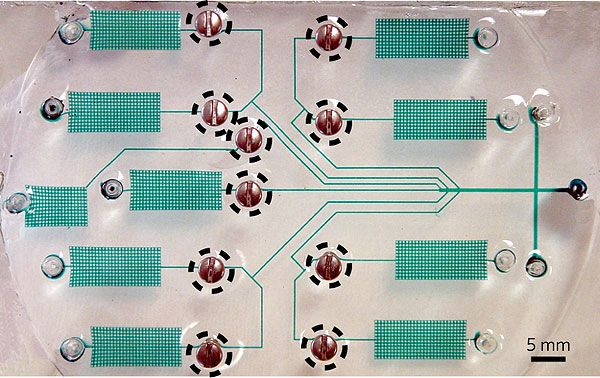
\includegraphics[width=\columnwidth,height=5cm,keepaspectratio]{Torque-immunoassay.jpg}
  \end{center}
  \caption{Coponents of a microfluidic device got increasingly complicated. This device from Ref.\citep{weibel2005torque} performs
  immunoassays - widely used in medical and biological research. The screws (dashed circles) are manually operated valves. Water with green dye
  shows the channels.}
  \label{fig:immunoassay}
\end{figure}


As these fabrication methods become more widely used the field of microfluidics moved, from
adding components to its analytical arsenal, to starting to find applications for devices.
Microfluidic devices then found applications in protein cyrstallisation \citep{hansen2002robust},
separations coupled with mass spectroscopy \citep{ramsey1997generating}, single cell manipulation \citep{wheeler2003microfluidic},
and synthesis of $^{19}$F-labelled organic compounds for use in PET scans \citep{lee2005multistep}.

A subsection of microfluidics began to emerge around this time too, as
low reynolds numbers make multiphase flow manipulation
relatively easy, the generation and manipulation of droplets\citep{thorsen2001dynamic, link2004geometrically, tan2004design} began to be explored.
These involved dispersing a liquid phase in a continuous
liquid stream to form a monodisperse emulsion of (often) aqueous droplets in oil. These droplets
were used to produce polymer particles\citep{nie2005polymer}, in making irregular particles\citep{nisisako2007formation},
hollow microcapsules\citep{utada2005monodisperse}, and protein detection in cells\citep{huebner2007quantitative}. An example of one of the ways droplets were first
produced in microfluidic devices is shown in \fig{fig:IntroDrops}.

\begin{figure}
  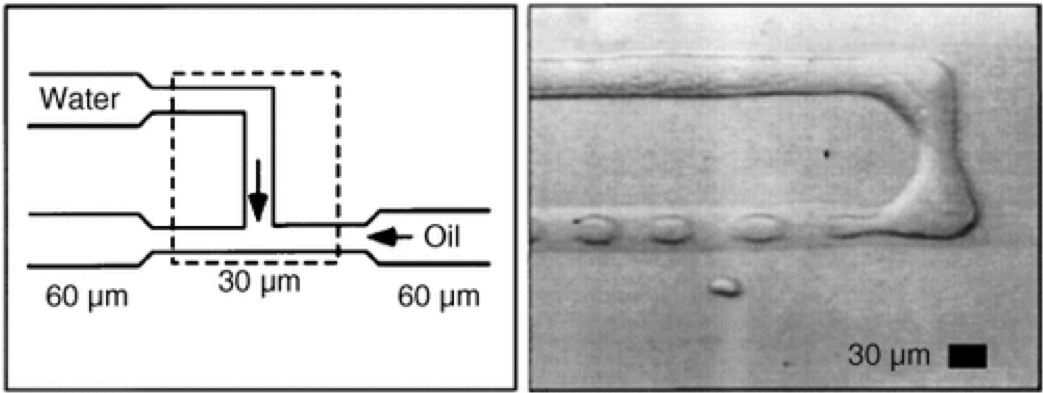
\includegraphics[width=\columnwidth]{Droplets.png}
  \caption{Formation of droplets in a T-Junction of a microfluidic device the continuous hydrocarbon
  phase disperses a water phase. Figure from \citep{RN104}}
  \label{fig:IntroDrops}
\end{figure}



In parallel, another branch of microfluidics was being developed. Its goal was to
culture cells in a repeatable way. In their normal environment, cells are subject to multiple
cues including cytokines and other signalling molecules from neighbouring cells, biochemical
interactions with the extracellular matrix, mechanical stress and direct cell to cell contacts.
Microfluidics was seen as an ideal method of providing cells with these cues in a controlled and reproducible fashion that couldn't be easily
replecated with conventional cell culture, by using microfludic devices one can combine
cell culture with analytical techniques in order to probe the biochemical processes that
govern cell behaviour.

\begin{figure}
  \begin{center}
  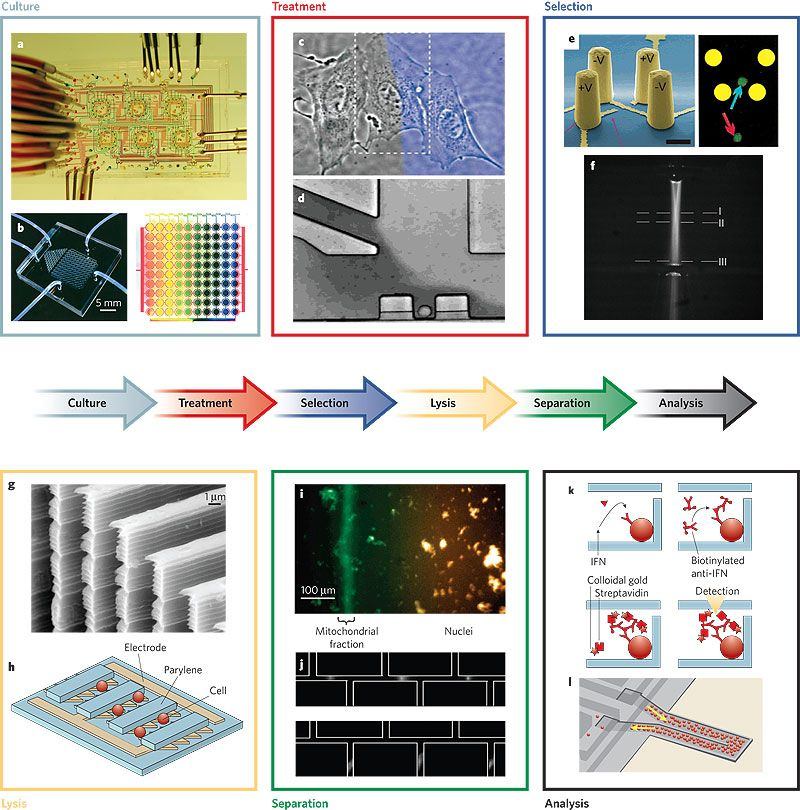
\includegraphics[width=\columnwidth,height=12cm,keepaspectratio]{Microfluidic-Cell-Culture.jpg}
  \end{center}
  \caption{A collection of microfluidic devices that enabled cell based assays from cell culture, to selection and treatment,
  to analysis. \textbf{a}, Six biorexctors are operated in parallel in a single chip to monitor small numbers of cells \citep{balagadde2005long},
  \textbf{b}, Microfluidic cell-culture array with integrated concentration gradient generator (left). Image of concentration
  gradient when blue and yellow dye is used (right) \citep{RN41}. \textbf{c} Two laminar streams exposing two sides of a single cell to different
  conditions \citep{takayama2001laminar}.
  \textbf{d}, Perfusion over a single trapped cell. The perfusion media can be switched in 100 ms \citep{wheeler2003microfluidic}. \textbf{e}, (left) Cell dielectrophoresis
  trap. (right) Fluorescent image of trapped cell indicated by blue arrow \citep{Voldman:2002gf}. \textbf{f}, Fluorescent image of light path at the detection
  zone in a micro flow cytometer \citep{wang2004measurements}. \textbf{g} Scanning electron micrograph of a mechanical lysis device with sharp knife-like protrusions \citep{di2003reagentless}.
  \textbf{h}, Schematic of electrical lysis device with microelectrodes \citep{lee1999micro}. \textbf{i}, Isoelectric focusing of cell organelles \citep{lu2004microfabricated}.
  \textbf{j}, Two-dimensional separation of four model proteins. Isoelectric focusing (top) followed by SDS gel electrophoresis \citep{li2004integration}.
  \textbf{k}, Schematic of immunoassay using microbeads as a solid support \citep{sato2002microchip}. \textbf{l}, Schematic of a hollow cantilever-mased mass sensor
  for analyte detection \citep{burg2003suspended}. Taken from Ref.\citep{el2006cells}}
  \label{fig:CellCulture}
\end{figure}


Microfluidic devices have been used enable cell-based assays from cell culture to biochemical analysis. In
\fig{fig:CellCulture} images of different devices are shown that convey how complex the devices being
produced were becoming, despite integration of functionalities proving difficult, these demonstrate the
power of miniaturisation and the ingenuity being developed in the field.
Microfluidics can offer unique control over cell-cell and soluble cues typical of
\textit{in vivo} cell environments by combining microfabrication of 3D extracellular matrix (ECM)
structres and fluid networks that can deliver nutrients and oxygen \citep{folch1999molding}.

Throughout the 2000s, microfabrication, which combined micropatterning techniques such as
photolithography, photoreactive chemistry, and soft lithography, made it possible to engineer the
microenvironment of the cell on similar length scales to the cell itself \citep{folch2000microengineering}. This surface
patterning of micrometre sized features enabled control of cell-EDM interactions and was used
to fabricate 3D scaffolds on which to grow cells that were made of biodegradable
materials \citep{tsang2004three}.

One area of application was the 3D culture of liver cells. \textit{In vitro} culture
of liver cells is of particular interest as many drugs fail clinical studies because they
either damaged the liver directly, or because the metabolites produced by the liver are toxic
\citep{sivaraman2005microscale}. Efforts were made to produce \textit{in vitro} culture
systems that mimic real liver conditions. In the liver, hepatocytes are found in a complex
3D environment in which nutrients, soluble factors and oxygen are transported through blood
capillaries and bile canaliculi. Using silicon as a substrate, Powers \textit{et al} fabricated
3D liver reactors using array of 300 µm wide channels \citep{powers2002microfabricated}. In their
device they perfused rat liver cells providing fluid shear stresses at physiological range. They found
that the cells seeded into the channels rearranged extensively to form 'tissue like' structures and
remained viable for up to 2 weeks.

Later, Sivaraman \textit{et al} developed a different system to culture liver cells in a 3D scaffold,
using a polycarbonate housing for a silicon device that contained microfabricated wells in which the
cells were seeded and perfused with media. They also found that the cells in the 3D culture
also had cell-cell contacts that resembled those found in tissues \textit{in
vivo} \citep{sivaraman2005microscale}. It has been observed that co-culture of hepatocytes with other cell types,
inculding liver epithelial cells and Kupffer cells, prolongs the survival of cultured hepatocytes and helps maintain
liver-specific properties such as albumin secretion \citep{guguen1983maintenance}.

As 3D cell culture became more widely used, a new subgenre of microfluidics was formed, organ-on-a-chip. Early efforts had shown
that microfabrication of adhesive substrates provided well-controlled environments for cell growth and epression of differentiated tissue-specific functions
\citep{chen1997geometric,bhatia1999effect}. Advances in soft lithography-based microfluidic devices made it easier
to develop the more complex 3D architecture of living tissues and organs. For example, a poly(dimethylsiloxane) (PDMS) device
that contained structures that mimic the structure of the endothelial-epithelial interface that forms the liver sinusoid \citep{nakao2011bile}.

Along with liver function, kidney, lung, and body functions were replicated in microfluidic devices shown in \fig{fig:OrganChip}. Whilst the liver and kidney offer highly
simplified microengineered models, within organs \textit{in vivo} nutrients, hormones, metabolites, cytokines and physical signals are usually transferred across interfaces
between adjacent living cells and therefore require a much more complex microenvironment
for true replication. Huh \textit{et al} created a model of the human alveolar-capillary interface formed in a flexible
PDMS device containing a central channel and two hollow side chambers \citep{huh2010reconstituting}. A 10 µm thick PDMS membrane containing an
ordered array of micropores (10 µm diameter) was stretched across the central channel, splitting it in two see \fig{fig:OrganChip}.
Human alveolar epithelial cells were then cultured on
one side of the membrane and exposed to air, while human lung capillary endothelial cells were cultured on the opposing side and exposed to flowing
medium. When the holllow side chambers were exposed to vacuum, the cells were subjected to strain ranging from 5\%-15\% to match strain observed within
whole lung \textit{in vivo}. In doing so, they found their 'lung on a chip' accentuated the inflammatory responses of the cells to silica
nanoparticles. This mechanical strain also enhanced uptake of nanoparticles and stimulated the transport into the vascular channel and
similar effects of physiological breathing were observed in whole mouse lung. These early organ on chip experiments paved the way for more complex
'Body-on-a-chip' devices that contain multiple types of cultured cells connected by a network of
microfluidic channels that permit recirculation and exchange of metabolites in a physiologically-relevant manner \citep{esch2011role} and
has found applications in drug screening and disease modelling \citep{skardal2016organoid}.


\begin{figure}
  \begin{center}
  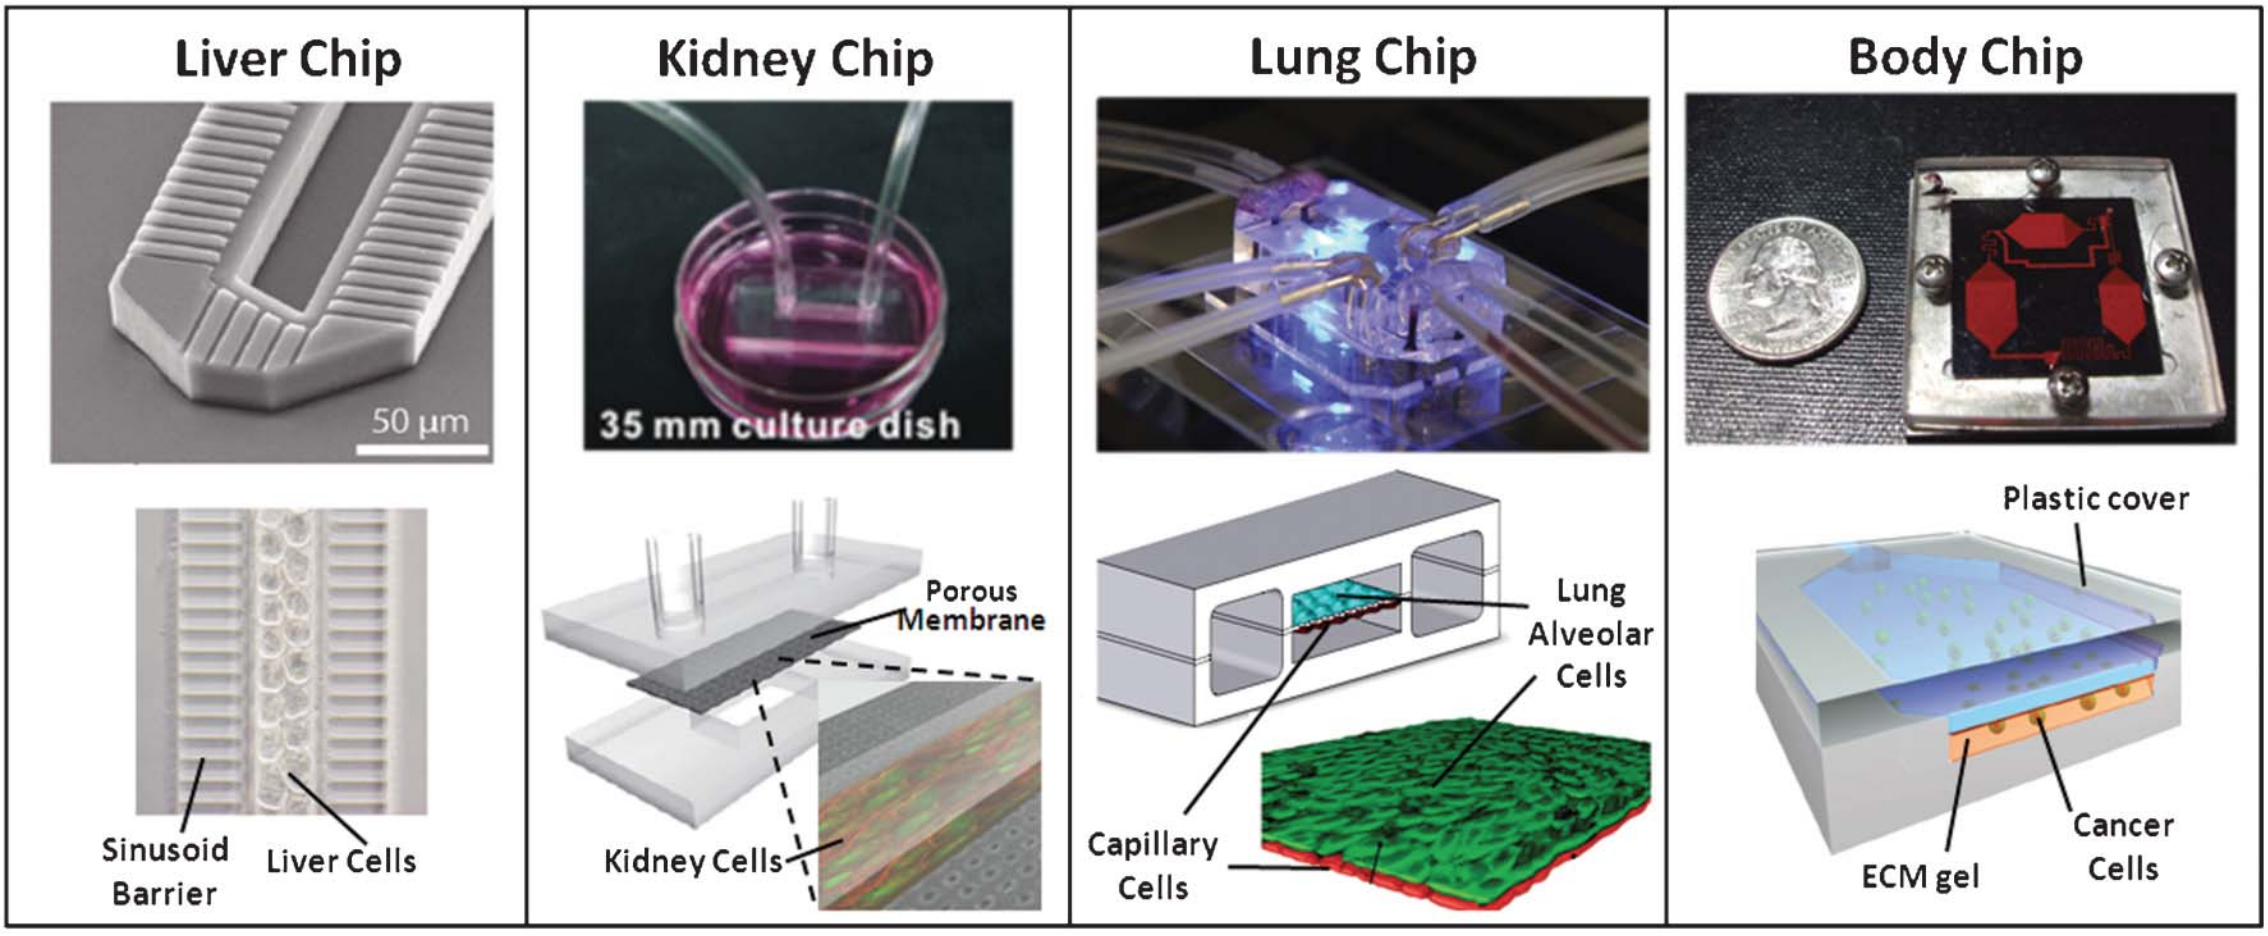
\includegraphics[width=\textwidth]{Organ-on-a-chip}
  \end{center}
  \caption{Organ-Organ and tissue-tissue interfaces in microdevices. Liver chip: A microfluidic liver device with cell culture and flow chambers separated by
  a baffle that separates cultured hepatocytes from fluid flow to simulate the endothelial-hepatocyte interface of the liver sinusoid. This geometry promotes alignment
  of hepatocytes in two lines that facilitates the production of functional bile canaliculi along hepatic-cord-like structures\citep{nakao2011bile}. Kidney chip:
  A simple kidney on a chip that mimics the interface between epithelium and flowing urine was created by donding a PDMS well and a PDMS channel to either side
  of a semi-permeable membrane on which cells are cultured and subejected to fluid flow\citep{jang2010multi}. Lung chip: A lung-on-a-chip capable of replicating mechanical
  strain caused by breathing, fabricated from PDMS that mimics the physiological function of the alveolar-capillary interface in the human lung. The hollow chambers
  are subjected to cyclic suction to replicate breathing movements whilst fluid flowing mimics blood flow\citep{huh2010reconstituting}. Body chip: A
  microfluidic device containing multiple linked tissue types representing different organs was conctructed by sealing three cell culture chambers against a cover. Each
  cell culture chamber contains a 3D ECM gel containing living cells from a different organ. Media was circulated through the chambers via microfluidic channels
  during operation\citep{sung2009micro}. Figure taken from \citep{huh2012microengineered}.}
  \label{fig:OrganChip}
\end{figure}

As the complexity of cell culture within microfludic devices increased, so to, did the detection methods. Coupling
a dector to an LOC is critical for any analytical purpose. A number of detector technologies were demonstrated in
microfluidic devices including electrochemical\citep{wang2006electrochemical}, mechanical \citep{raiteri2001micromechanical},
and optical methods \citep{kuswandi2007optical}. The small sample volumes typical to a microlfuidic experiment
are an important challenge to overcome for any detector, ideally, a detector should be highly sensitive and scalable
to smaller dimensions.

The mechanism and features of the detection technologies summarised in \citep{pires2014recent} and
reproduced in Table \ref{tab:detectors}.

\newpage

\begin{table}
\begin{center}
    \label{tab:detectors}
    \begin{tabular}{|p{5cm}||p{5cm}||p{5cm}|}\hline\hline
      Method & Mechanism & Features \\ \hline
      Electrochemical & Measures changes in conductance, resistance and/or capacitance at the active surface of the elctrodes  &
      (+) Real-time detection, (+) Low-cost microelectrode fabrication, (-) Control of ionic concentrations before detection, (-) Short sehelf life  \\ \hline
      Mechanical & Detection is based on variations of the resonant frequency or surface stress of the mechanical sensor &
      (+) Monolithic sensor integration, (+) Label free detection, (-) damping effects in liquid samples, (-) Detection takes time (~30 mins), (-) Complex fabrication  \\ \hline
      Optical & Detects variations in light intensity, refractive index sensitivity, or interference pattern &
      (+) Minimal sample preparation, (+) Real-time detection, (+) Ubiquitous in laboratories, (-) Conventional instrumentation is expensive, (-) Set-up complexity \\ \hline\hline
    \end{tabular}
\caption{Summary of electrochemical, mechanical and optimal deteciton technologies employed in microfluidics.}
\end{center}
\end{table}

Electrochemical detection involves the interaction of chemical species with electrodes or probes. This interaction
results in a variation of signal, such as potential or current, which enables analysis of target analytes. The
electrochemical phenomenon deals with two major effects: (i) chemical reactions are promoted by passing an
electrical current through the electrode system; or (ii) electrode responses are triggered due to specific chemical reactions. These
effects are usually observed using an eletrolytic cell. Reactions of oxidation and reduction occurring at the surface of the electrodes
are the basis for electron transfers between the electrolyte (sample) and the electrodes. In a typical
electrolytic cell, the electrode system is formed by the working electrode where detection of a certain
analyte is analyzed, and the reference electrode where a standard oxidation/reduction is conducted \citep{flanagan2005electrochemical}.
Wongkaew \textit{et al} reported an electrochemical biosensor that employed microelectrode array. In
the array, adjacent electrode fingers form micro-sized gaps which allow an increase of the diffusion flux
of chemical species, thus leading to an enhanced collection efficiency and higher signal amplification.
The microchannels of the device were made by hot embossing PMMA and the electrodes were made by e-beam
and wet-etching processes. The detection of targets using this system took 250 seconds and reported
limit of detection of 12.5 µM.

Mechanical detection systems mainly used cantilever technology, which showed that it could be accurate
when detecting biomolecules \citep{waggoner2007micro}. Cantilever-based devices generally operate in two
different modes upon analyte binding: (i) static deflection, where binding on one side of a cantilever
causes unbalanced surface stress resulting in a measurable deflection; (ii) dynamic, resonant mode, where
binding on a cantilever causes variations of its mass and consequently shifts the resonant frequency.
Mechanical-based detection may require no labelling of biomolecules. Labels often make the detection
method more complicated, time-consuming and costly, and could interfere with the function of biomolecules
under investigation. Anoter characteristic of cantilever technology is the potential to fabricate large
arrays of sensors for multi-molecular sensing \citep{ferrari2005cancer}. Hou \textit{et al} \citep{hou2013aptamer} presented
a device that contained a microfabricated canter lever array  for the  specific detection of
oxytetracycline (OTC), a common broadband antibiotic used in animals that can accumulate in our food chain
and cause side effects on humans. The device achieved this by functionalising the cantilvers with OTC
specific DNA aptamers which bind to the OTC and icrease the load on the cantilevers and causes them
to deflect and once calibrated can indicate the concentration of OTC in solution. The limit of detection
in this case is 0.2 nM in 1000 seconds.

Optical detection is preferred for robust, sensitive Lab on a chip devices it has been the most widely
used technique for quantitative proteomic analysis \citep{rusling2010measurement} and infectious disease
diagnostics \citep{foudeh2012microfluidic}, due, in part, to the ubiquity of the optical instrumentation
required in biological laboratories meaning these devices can be used readily in most locations.
Conventional optical detection methods, including absorbance \citep{wang2011integration},
chemiluminescence \citep{wojciechowski2009organic}, fluorescence \citep{yildirim2012aptamer}, and surface
plasmon resonance (SPR) \citep{foudeh2014sub}, have all been applied in microfluidic devices. Foudeh
\textit{ et al} \citep{foudeh2014sub} developed an SPR microdevice for the detection of
\textit{Legionella pneumophila} which is the pathogenic organism that causes Legionellosis, and
is responsible for fatality rates over 10\% within hospital and indutrial outbreaks
\citep{swanson2000legionella}. The device is ultra-sensitive to RNA of \textit{Legionella pneumophila}
and has a limit of detection of 1 pM in less than 3 hours.

Presently, Microfluidics is a large and diverse field, so much so that the areas that started out as sub-categories are now referred to as their
own field of research, indeed, within the last three years the journal Lab on a Chip has published no less than 116 reviews focusing on a wide variety of applications
that microfluidics now enjoys such as: 3D printed fluidic networks\citep{kinstlinger20163d}; droplet microfluidics for synthetic biology\citep{gach2017droplet};
phase behaviour characterization for industrial CO$_2$, oil and gas\citep{bao2017microfluidic}; the production of stem cells using messenger RNAs\citep{giulitti2019direct};
and paper microfluidics for diagnosis of malraia in low resource community\citep{reboud2019based}.


\subsection{Goal}

Microfluidics is a broad term that covers a wide variety of research, it is characterised by
the analysis of small volumes of liquids usually nL to $\mu$L, in doing so, it offers numerous benefits
such as: a reduction in the materials used in experiemnts which leads to less cost and less waste; a high
level of control over the microenvironment; and ease of parallelisation and automation.
Microfluidics chiefly uses Lab-on-a-chip (LoC) devices, or micro total analysis
systems (µTAS), to perform experiments. These devices, or systems, are intended for the of scaling down of
labratory functions to a chip-format, the sizes of which range from a few mm$^2$ to a few cm$^2$.

Currently, NMR spectroscopy is not widely utilised in microfluidic devices, or experiments, and could be
used to provide extra information on the system. It can also be used in conjunction with existing methods
of analysis in microfluidics such as fluorescence spectroscopy.
As NMR leaves the sample unpeturbed, this makes it an ideal candidate for \textit{in situ} monitoring of
living systems.

The goal of the work presented here is to incorporate functional microfluidic experiments with high
resolution NMR spectroscopy, in such a way that the validity of either section, microfluidic or magnetic
resonance, remains intact. In this approach, microfluidic capability is preserved by utilising a design
that, whilst constrained by size and shape, has freedom to house a wide variety of chip designs that enable
a host of applications, a few of which are shown in \fig{fig:DifferentChips}. This means that functional
microfluidics can be performed, and coupled, with high resolution NMR spectroscopy. In this way not only
could NMR become a more widely used tool in the microfluidic toolbox, it would also make a valuable
attachment to existing tools

High resolution NMR spectroscopy itself requires an extremely homogenous magnetic field, this means that
any device capable of combining microfluidics and NMR should seek to preserve the homogeneity. This combination, however, is not without significant challenges. Firstly, a probe capable of µNMR must
be designed with comparable performance to existing probes, to maintain validity, and work with existing
magnets and spectrometers. Secondly, the chip, and any functionality it possesses must fit in the bore of
the magnet which is typically around 38 mm in diameter. This chip should also couple to the probe in a
removable way to enable parallelisation of experiments, preserving one of the key attributes of microfluidics.
Thirdly, the materials used in construction should be non-magnetic wherever possible and the use of magnetic
parts should be kept to a minimum. When designing experiments, the magnetic susceptibilities of solutions and
chip material should also be considered as these need to be as closely matched as possible in order to preserve
spectral resolution (a solution for when this isn’t the case is discussed in chapter \ref{Chapter:Droplets}).


\begin{figure}
  \begin{center}
  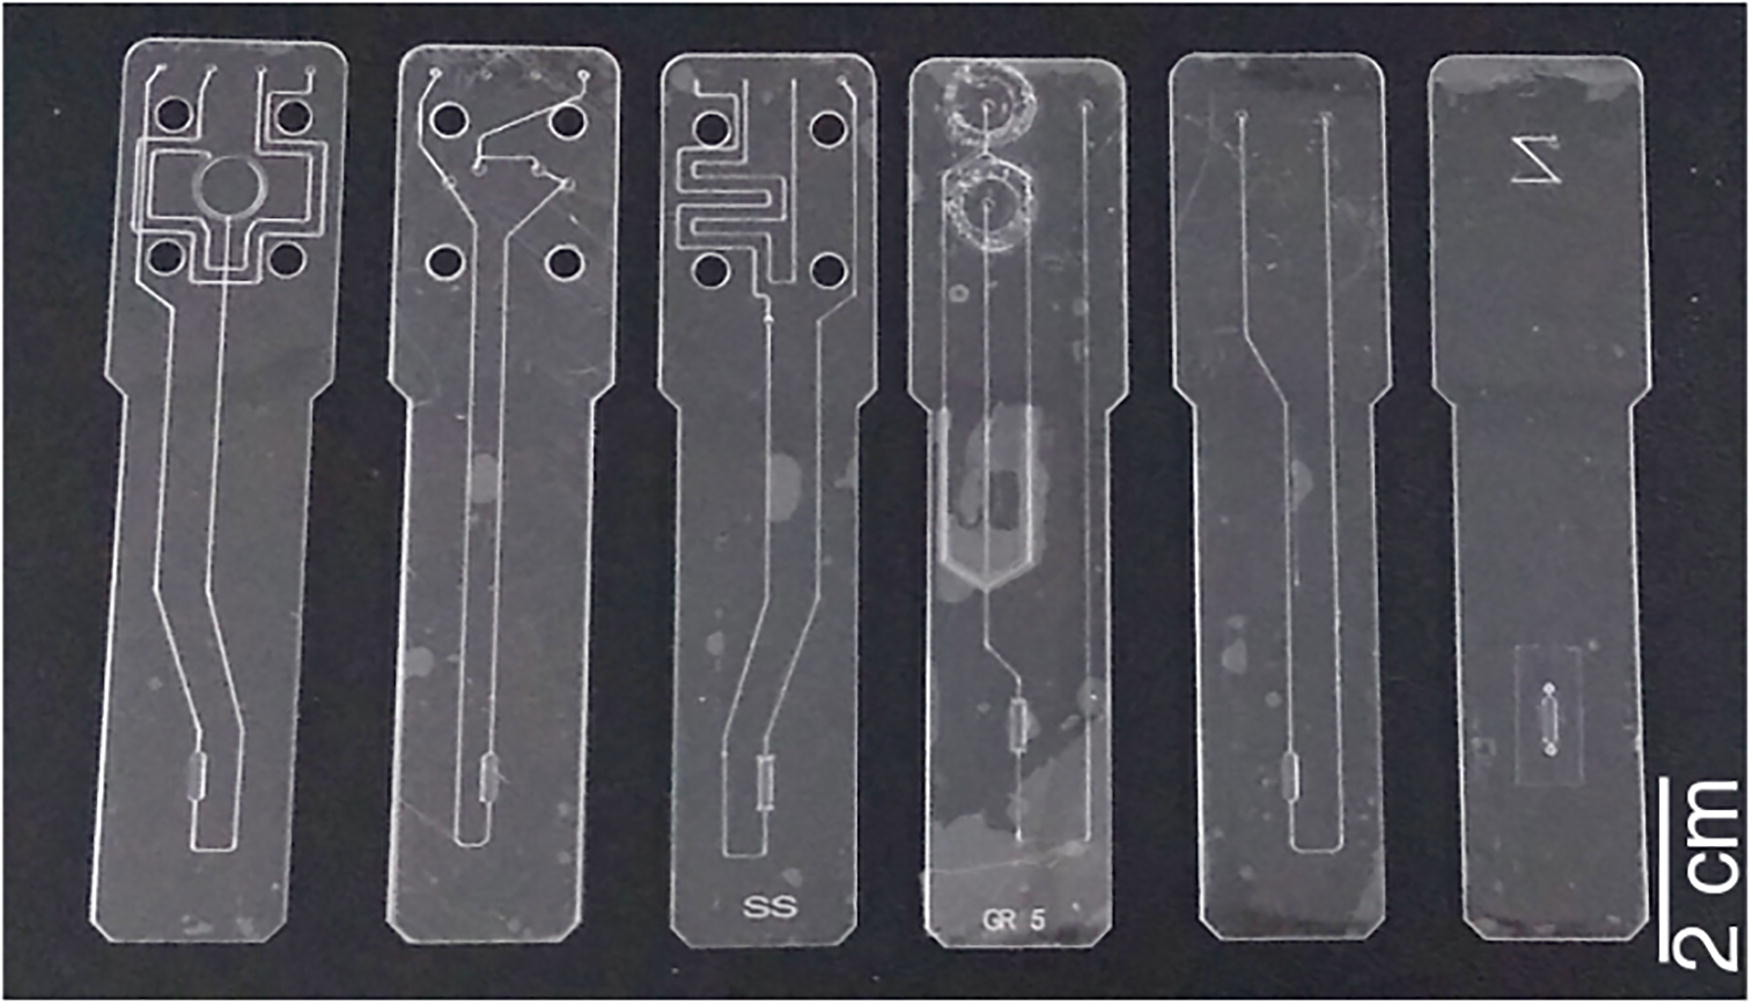
\includegraphics[width=\textwidth]{MVChips.jpg}
  \end{center}
  \caption{Microfluidic devices developed for this work, as well as for other applications in microfluidic
  NMR. From the left: A device for perfusion culture of a tissue slice on chip; capable of peristaltic
  pumping; hydrogenation on a chip; droplet generation; simple sample chamber filler; 2D/3D cell culture
  device. Figure taken from \citep{RN164}}
  \label{fig:DifferentChips}
\end{figure}

By combining these two fields, and harnessing the 'best of both worlds' approach
new insight and analysis is available. Having quantitative, system-level information in a
a single or just a few scans could benefit a wide variety of experiments. Enabling microfluidic
NMR also provides the oppurtunity to scan mass-limited samples such as those commonly found in
ligand binding reactions\citep{Finch:2016gv} or macrocyclic chemistry\citep{RN81}.

\newpage

\section{NMR theory}

Nuclear magnetic resonance (NMR) theory can be described using two approaches:
\begin{enumerate}
  \item The classical approach, in which the the nuclei are thought of as small bar magnets which
  rotate in 3D space. Experiments can be described be approxiamating the net magnetisation as a
  vector in 3D space.
  \item The quantum mechanical approach, in which each spin in the system is in a distinct quantised state.
  Operators are used to describe the state of a system as a whole. Experiments are described by propagating
  these operators.
\end{enumerate}

The theory described in this chapter is mainly from \citep{RN135,RN136} and is intended to provide sufficient background
knowledge in order for the reader to understand later chapters.

\subsection{Classical NMR}

\subsubsection{Spin}

Atoms, often modelled as a clump of neutrons and protons at
the centre known as the nuceleus, surrounded by electrons, have a property reffered to as spin.

In fact, nuclear spin is an intrinsic property of the nucleus and can take half or whole
integer values, including $0$. In this thesis one spin- 1/2 nucleus, the proton ($\ce{^{1}H}$) will be discussed, with another spin-1/2 nucleus \ce{^{13}C} making
sparse appearences. Just like in this thesis, $\ce{^{13}C}$ only has an $\approx{1}\%$
abundance in nature with the other $\approx{99}\%$ $\ce{^{12}C}$ having a spin-$0$
nucleus.

All spin-1/2 nuclei possess a magnetic dipole moment and behave rather like small bar magnets in that, when placed in an external magnetic field they have a tendency to align
with the field. In NMR this external field is called $B_0$, and is orientated along the
$z$-axis.

\subsubsection{Population}\label{Population}

In a magnetic field, a spin-1/2 nucles has two energy levels with a separation that is proportional to the strength of the magentic field, a schematic is show in \fig{fig:EnergySplit}. We label these levels $\alpha$ and $\beta$.

\begin{figure}
  \begin{center}
  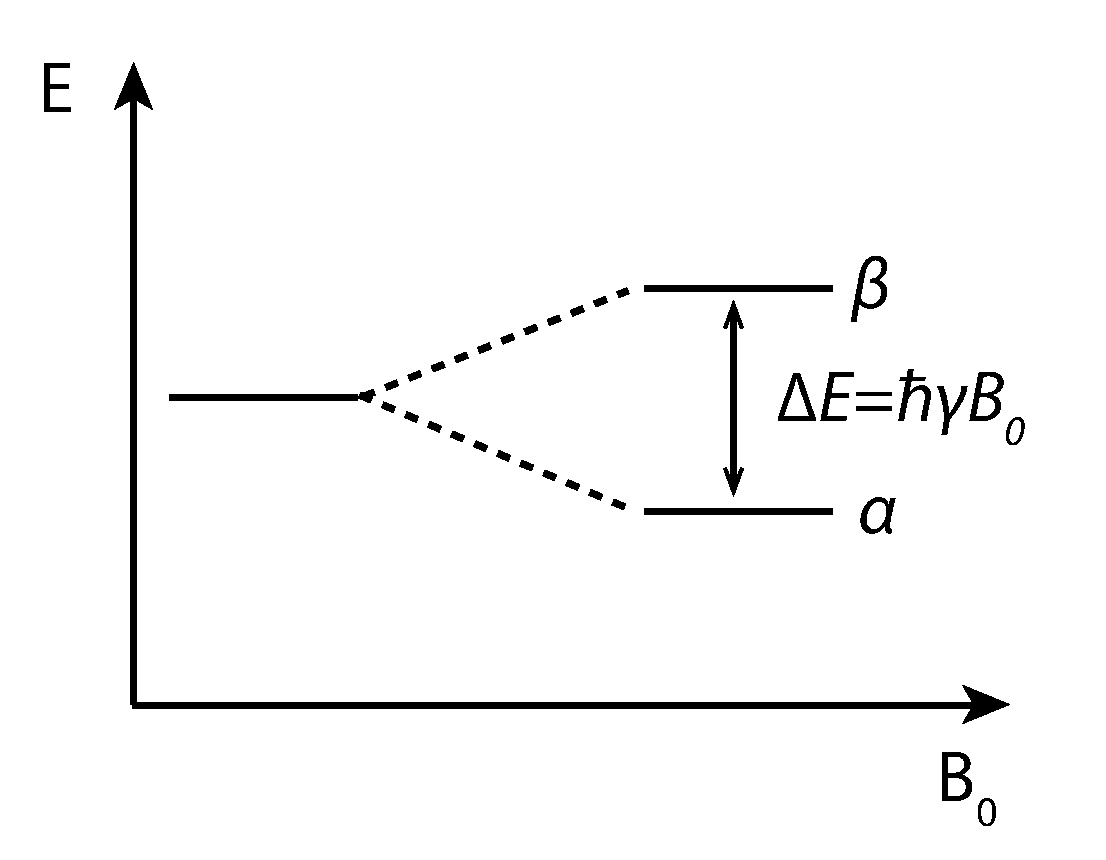
\includegraphics[width=\textwidth,height=5cm,keepaspectratio]{EigenStateLevel.pdf}
  \end{center}
  \caption{Energy level and $\Delta~E$ of the two energy levels for a spin-1/2 nucleus}
  \label{fig:EnergySplit}
\end{figure}

When measuring a group of spins, each spin can exist in either the $\alpha$ or $\beta$ state and overall
the spins have a slight preference for the lower energy state, $\alpha$. This preference can be quantified
by calculating the difference in populations ($P$) which at thermal equilibrium is governed by the
Boltzmann distribution:
\begin{equation}\label{eqn:Boltzmann}
  \frac{P_{\beta}}{P_{\alpha}} = \text{exp}\{\frac{-\Delta{E}}{k_B T}\}
\end{equation}

where $P_{\beta}/P_{\alpha}$ is the population ratio between the states, $k_B$ is Boltzmann constant, and $T$ is the temperature. The polarisation, $p$, of a system of
spin-1/2 nuclei is
\begin{equation}\label{eqn:Polarisation}
  p = \frac{P_\alpha - P_\beta}{P_\alpha + P_\beta}
\end{equation}

For a system in an NMR experiment which typically operates at 298$K$ and
a field of 14.1 T the polarisation level is circa $10^{-5}$ meaning That the spins are aligned weakly in the same direction as the magnetic field. It is this small polarisation that gives rise to the NMR signal and why NMR is famed for sensitivity
issues. One possible solution to this, hyperpolarisation, will be described in a later chapter.

\subsubsection{Nuclear spin precession}

When placed in a magnetic field, the nuclei will precess around the axis of the field at a rate known as the larmour frequency defined as:
\begin{equation}\label{eqn:larmour}
  \omega_j^0 = -\gamma_jB_0
\end{equation}

where $\gamma_j$ is the gyromagnetic ratio for a nucleus, $j$. The gyromagnetic ratio is
typically $10$s of MHz T$^{-1}$ that give larmour frequencies in the $100$s of MHz in an NMR
experiment.

\subsubsection{Magnetisation as a vector}

The net magnetic moment of a spin ensemble can be modelled by a 3D vector that can rotates in space. The essence of this is shown in \fig{fig:VectorFig}. Magnetisation is intially taken to be orientated along the $z$-axis, this is called longitudinal magnetisation. It is then rotated into the $xy$-plane which is called transverse
magnetisation that then precesses about the $z$-axis.

\begin{figure}
  \begin{center}
  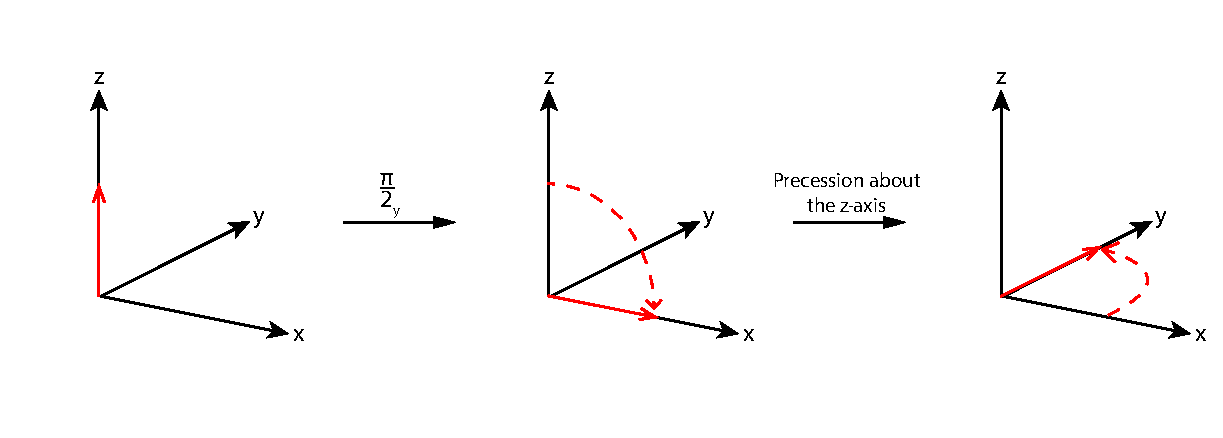
\includegraphics[width=\textwidth]{VectorFig.pdf}
  \end{center}
  \caption{Magnetisation shown as a vector in red, at equilibrium, is orientated on the $z$-axis. A $pi$/2
  pulse rotates the vector to the $xy$-plane where it begins to precess around the $z$-axis.}
  \label{fig:VectorFig}
\end{figure}

How this vector changes in a magnetic field is described using the Bloch equations\citep{Bloch:1946hk}. These are a group of differential equations that
describe how the magnetisation vector components evolve in time in the
presence of orthogonal magnetic fields.
\begin{align}\label{eqn:Bloch}
  \frac{dM_x(t)}{dt}\quad=\quad\gamma(M_y(t)B_z(t)-M_z(t)B_y(t))\\
  \frac{dM_y(t)}{dt}\quad=\quad\gamma(M_z(t)B_x(t)-M_x(t)B_z(t))\\
  \frac{dM_x(t)}{dt}\quad=\quad\gamma(M_x(t)B_y(t)-M_y(t)B_x(t))
\end{align}
where $M_a$ is the magnetisation vector component along the $a$-axis, $B_a$ is the
magnetic field along the $a$-axis, and $\gamma$ is the gyromagnetic ratio as described before.

In the case of processing magnetisation around the $z$-axis, here denoted $B_0$, the
Bloch equations can be written as
\begin{align}
  \frac{dM_x(t)}{dt}\quad=&\quad\gamma~B_0M_y(t)\\
  \frac{dM_x(t)}{dt}\quad=&\quad-\gamma~B_0M_x(t)\\
  \frac{dM_x(t)}{dt}\quad=&\quad0
\end{align}
these have the solutiion
\begin{align}
  \frac{dM_x(t)}{dt}\quad=&\quad\cos(\omega^0t)M_x(0) + \sin(\omega_0t)M_y(0)\\
  \frac{dM_x(t)}{dt}\quad=&\quad\cos(\omega^0t)M_y(0) + \sin(\omega_0t)M_x(0)\\
  \frac{dM_x(t)}{dt}\quad=&\quad0
\end{align}
where $\omega^0$ is the larmour frequency from \eqn{eqn:larmour}.

\subsubsection{Pulses and rotating frame}

\subparagraph{Rotating frame}

The field, $B_0$, of a regular NMR experiment is many Tesla, giving precession
frequencies of hundreds of megahertz. These frequencies correspond to radio frequencies in the electromagnetic spectrum. When considering these precessing spins
it can be useful to change from a static frame to a rotating frame of reference.

The general case is when the rotating frame is at frequency $\omega_{rot}$, in this
frame, the larmour frequency will appear to be ($\omega - \omega_{\text{rot}})$. This is called the offset,$\Omega$ and is given by:
\begin{equation}
  \Omega = \omega -\omega_{\text{rot}}
\end{equation}

It follows from this, that if the apparent larmour frequency in the rotating frame is different from that in the static frame, it must also be the case that the apparent magnetic field in the rotating frame must be different from the applied
field. We can use \eqn{eqn:larmour} to compute the apparent magnetic field, $B^{\text{red}}_0$:
\begin{align}\label{eqn:redB}
  \Omega =& -\gamma~B^{\text{red}}_0\\
\text{hence}\quad~B^{\text{red}}_0 =& \frac{\Omega}{\gamma}
\end{align}
this apparent magnetic field in the rotating frame is called the reduced field, $B_{\text{red}}$.

\begin{figure}
  \begin{center}
  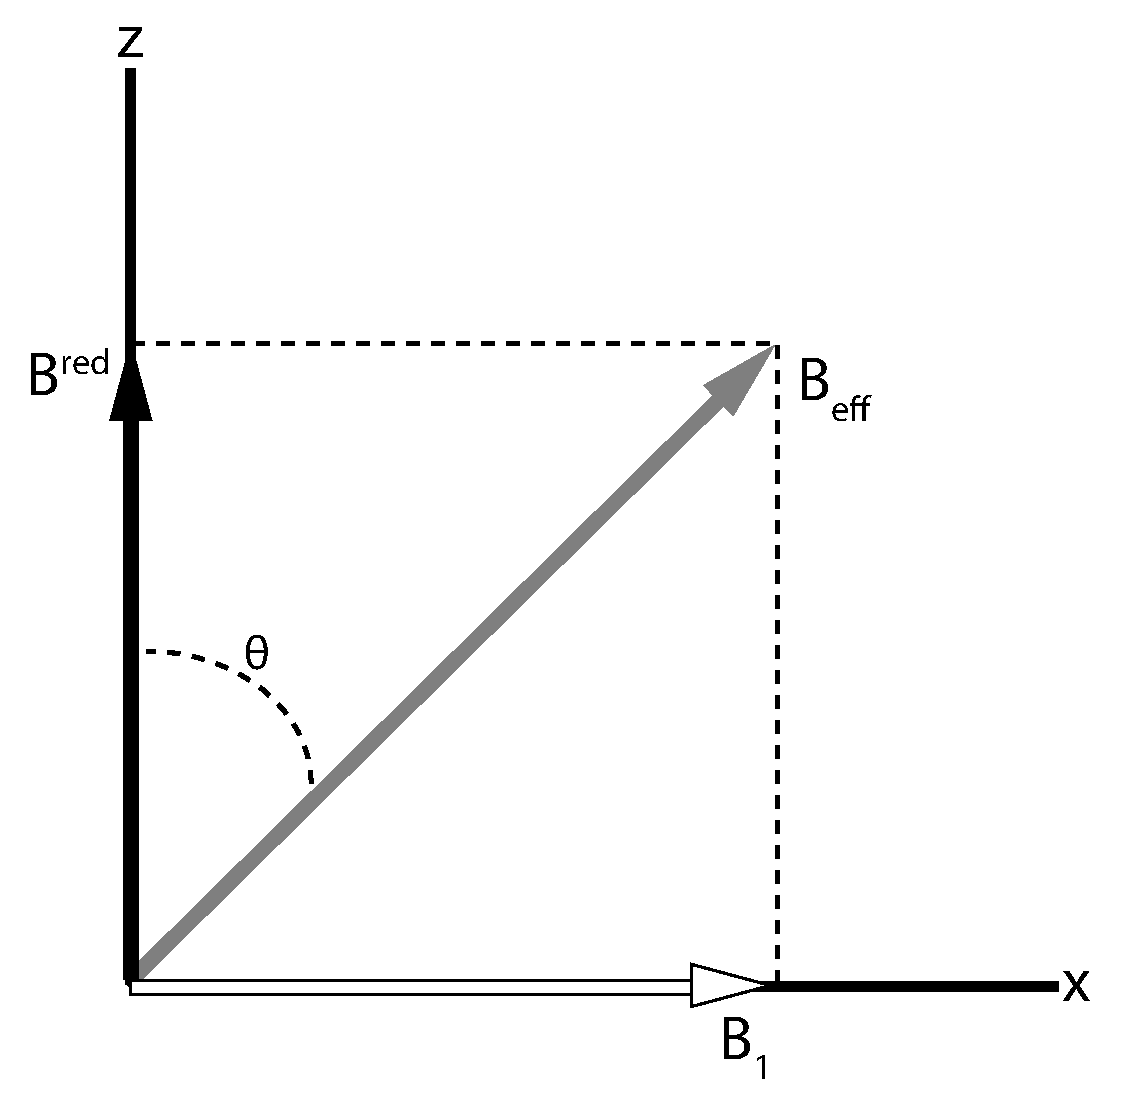
\includegraphics[width=\textwidth, height=7cm, keepaspectratio]{B1Bred.pdf}
  \end{center}
  \caption{In the rotating frame the effective field, $B_{\text{eff}}$, is the vector sum of the reduced field,
  $B_{\text{red}}$ and the $B_1$ field. $\theta$ is the tilt angle defined between $B_{\text{red}}$ and $B_{\text{eff}}$}
  \label{fig:BMag}
\end{figure}


\subparagraph{Pulses}

In NMR experiments, pulses are used to manipulate magnetisation in order to obtain a signal. A pulse can be
thought of as a magnetic field oscillating at the frequency of the rotating frame
applied in the $xy$-plane in order to induce procession of the magnetisation. This magnetic field is labelled $B_1$ and is much smaller in amplitude than $B_0$, the actual applied field.

\begin{figure}
  \begin{center}
  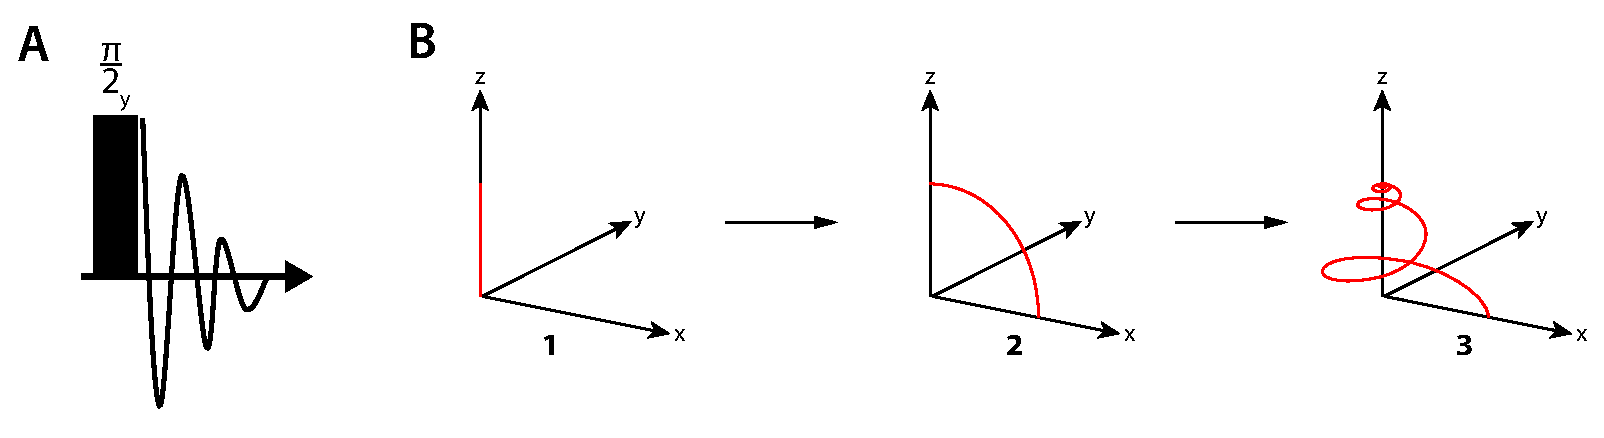
\includegraphics[width=\textwidth]{SpinRelaxation.pdf}
  \end{center}
  \caption{A) A graphical representation used to describe a pulse sequence, the width and height of the block
  refer to the power and duration of pulse respectively, the line represents the acquisition of signal. B)(1) The
  magnetisation lies in equilibrium along the $z$-axis. (2)  The $\pi/2_y$ pulse rotates the magnetisation around the $y$-axis. (3) The magnetisation precesses in the $xy$-plane around the $z$-axis and returns to thermal equilibrium}
  \label{fig:Pulse}
\end{figure}

In the static frame, the magnetisation is processing around $B_0$ at the larmour frequncy, so a relatively weak $B_1$ applied along the $y$-axis, for example, would do little to peturb it, given the effective magnetic field, $B^{\text{eff}}_0$, is calculated by:
\begin{equation}
  B^{\text{eff}}_0 = \sqrt{(B_1)^2+(B_0)^2}
\end{equation}
the much larger $B_0$ dominates here, however, if we apply the $B_1$ in the rotating
frame this becomes
\begin{equation}
  B^{\text{eff}}_0 = \sqrt{(B_1)^2+(B^{\text{red}}_0)^2}
\end{equation}
and using \eqn{eqn:redB} as $\omega_{\text{rot}}\rightarrow\omega$, $\Omega\rightarrow0$ and $B^{red}_0\rightarrow0$ so by making the offset small, or zero, the effective field
then lies close to the $xy$-plane and so the magnetisation will be rotated down
from $z$ which is what we'd like to acheive for our experiments.

The key, is that although $B_0$ is much larger than $B_1$, we can still affect magnetisation using $B_1$ by making it oscillate close to the larmour frequency
this is the phenomena of resonance. The angle between $B^{\text{red}}_0$ and $B^{\text{eff}}$ is
called the tilt angle, $\theta$. It can be seen from \fig{fig:BMag} that:
\begin{equation}
\sin(\theta) = \frac{B_1}{B_{\text{eff}}}\qquad\cos(\theta) = \frac{B^{red}_0}{B_{\text{eff}}}\qquad\tan(\theta) = \frac{B_1}{B^{\text{red}}_0}
\end{equation}

These radio frequency (rf) pulses are useful because they can be used to address spins at a specific larmour
frequncy. By applying an rf pulse on resonance with $\ce{^1H}$ we can manipulate the magnetisation of the nuclei whislt not affecting other spins (e.g. $\ce{^13C}$) contained in the sample.

\subsubsection{Fourier Transform NMR}

In this section we will examine how we can produce an NMR spectrum from the magnetisation of a sample
using the rf pulses we introduced.

In NMR we use a pulse sequence to describe the intensity and duration of pulses used in an
experiment, shown in \fig{fig:Pulse}. The rf pulse, $B_1$, is a $\pi/2$ pulse in the $y$-axis, followed by a signal
acquisition. This pulse tips the magnetisation into the $xy$-plane, and if the pulse length is much less than the
precession period (we will assume so), the spins begin to precess freely around the $z$-axis at the larmour
frequency, $\omega_0$, until they return to the $z$-axis through a process described in \ref{Relaxation}.

In a usual NMR experiment the signal is inductally detected. The oscillation of the spins in the sample induces
a current in the pick-up coils around the sample, which is detected, amplified and transformed into a spectrum.
The resulting free induction decay (FID) is typically an exponentionally decaying sinusoidal function. The signal
produced from this can be written as:
\begin{align}\label{eqn:signal}
  S(t) =& \sum_l s_l(t) \\
  s_l(t) =& a_l\text{exp}\{-(i\omega_l+\lambda_l)t\} = a_l(\cos(\omega_lt) + i\sin(\omega_0t))\text{exp}\{-\lambda_l~t\}
\end{align}
where $S(t)$ is the total signal from from the sample and $s_l$ are the individual spins. Each spin has an amplitude, $a_l$, and an associated decay constant, $\lambda_l$. The nature of which will be discussed in \ref{Relaxation} section. Exponential to trigometric function conversion
is done according to Euler's formula: $\text{exp}\{ix\} = \cos(x) + i\sin(x)$.

$S(t)$ is easy to evaluate and interpret if it originates from one spin or a group of spins precessing
at precisely the same frequency, however, if there are more spins in the sample processing at different frequencies
the FID becomes extremely hard to interpret on its own.

We can clear this picture up however by employing a Fourier transform. This comverts the time-domain data
into the frequncy-domain, such that the total signal in the frequency domain, $S(\omega)$ is the sum of all individual spin signals in the frequency, $S_l(\omega)$:
\begin{equation}
  S(\omega) = \sum_l S_l(\omega)
\end{equation}
This allows us to clearly see which resonances are possessed by our spins in the sample. To
perform a Fourier transform we must do the following:
\begin{equation}
  S_l(\omega) = \int_{0}^{\infty}s_l(t)\text{exp}\{-i\omega t\}dt
\end{equation}
and using \eqn{eqn:signal} can be rewritten:
\begin{equation}
  S_l(\omega) = a_l\int_{0}^{\infty}\text{exp}\{(-i(\omega+\omega_l)+\lambda_l t\}dt
\end{equation}
sometimes written more concisely as:
\begin{equation}
  S(\omega) = \mathcal{F}\{S(t)\}(\omega)
\end{equation}
where $S(t)$ is the signal for the time domain (FID) and $S(\omega)$ is the signal in the frequency domain.

The Fourier transform of our general case is:
\begin{equation}
  \mathcal{F}\{S(t)\}(\omega) = a_l\frac{1}{\lambda_l + i(\omega - \omega_l)}
\end{equation}
which is Lorentzian function centered at $\omega_l$ with peak width parameter $\lambda_l$.

The NMR signal represented in the frequency domain is a spectrum. It is usually many peaks
indicating different resonance frequencies of spins in the sample. In the next
section we will discuss chemical shift and J-coupling. Two additional effects that when combined
with larmour frequencies already discussed forms the NMR spectrum as we know it.

\subsubsection{Chemical Shift and J-coupling}

In a molecule, nuclei are surrounded by clouds of electrons which can shield, or de-sheild, it
from the effects of the external field $B_0$.

The chemical shielding factor, $sigma$, shifts the resonance frequency of the nuclear spin. We
can now include it in \eqn{eqn:larmour}:
\begin{equation}
  \omega_j^0 = -\gamma_jB_0(1-\sigma)
\end{equation}
this chemical shielding is specific to each nucleus in the molecule. It is possible
for two or more nuclei to share the same factor. We refer to these as being chemically equivalent.

The shielding is often around $10^-6$ for $\ce{^1H}$. When plotting and examining spectra
it is would not be useful to use absolute frequecies, as discussed they are regualarly in the hundreds of MHz,
whereas the differences in peaks might only be kHz or less. To combat this we use a relative frequency scale
called chemical shift, $\delta$, it is defined as:
\begin{equation}
  \delta = \frac{\omega_j-\omega^\text{ref}_j}{\omega^\text{ref}_j}
\end{equation}
where $\omega_j$ is the precession frequency of the nucleus of interest, and $\omega^\text{ref}_j$ is the precession
frequency of a reference nuclei. $\delta$ is a dimentionless number, unaffected by magnetic field strength, it often
small compared to the size of the field and is reported in parts per million (ppm).

In addition to the external $B_0$ field, the nuclear spins are also affected by the magnetic fields generated
by neighboring spins. These magnetic fields are mediated by the electrons in the chemical bonds. This is refered to as
spin-spin couling or $J$-coupling and gives rise to peak splittings in spectra. These splittings, and therefore the values of $J$-couplings, range from a few Hz to a thousand Hz typically. It is an important factor and is icorperated
in the quatum description on NMR in \ref{Hamiltonian}.

Both of these, $\sigma$ and $J$-couplings, are tensors this means they depend on the orientation of the molecule
and the spin with respect to the magetic field. In liquids, however, tumble rapidly compared to the timescale
of an NMR experiment. This averages the interactions resulting in a scalar quantity for each.

There are additional effects the nuclear spins experience, for example, dipole-dipole coupling which
is a through space spin-spin coupling, and quadrapole coupling where there are spins with >1/2 values
however, these are not relevant to this work.

\subsubsection{Relaxation}\label{Relaxation}

The last part needed to complete our classical understanding of NMR is relaxation. Relaxation is the process
of the spin returning to the thermal equilibrum. The thermal equilibrium of spin-1/2 nuclei in a
magnetic field is the bulk magnetisation vector pointing in the direction of the $B_0$ field.

In this system there are two forms of relaxation, $T_1$ and $T_2$. $T_1$ is the longitudal relaxation time
constant and $T_2$ is the transverse relaxation time constant the difference between them is shown in \fig{fig:t1t2}.
$T_1$ is the rate constant that governs the return of magnetisation to the $z$-axis from the $xy$-plane. $T_2$ on
the other hand is the time constant that governs the return of magnetisation to equilibrium in the $xy$-plane.
It is more accurate to say that $T_1$ is the relaxation rate constant for populations, and $T_2$ is the relaxation
rate constant coherences, in the density operator (discussed in \ref{Quantum}). But this is incompatible
with the classical description of NMR.

We can now complete the Bloch equations from \eqn{eqn:Bloch}:
\begin{align}
  \frac{dM_x(t)}{dt}\quad=&\quad\gamma(M_y(t)B_z(t)-M_z(t)B_y(t)) - \frac{M_x(t)}{T_2}\\
  \frac{dM_y(t)}{dt}\quad=&\quad\gamma(M_z(t)B_x(t)-M_x(t)B_z(t)) - \frac{M_y(t)}{T_2}\\
  \frac{dM_z(t)}{dt}\quad=&\quad\gamma(M_x(t)B_y(t)-M_y(t)B_x(t)) - \frac{M_z(t)-M_0}{T_1}
\end{align}
in order to derive $M_{xy}$ we assume the following:
\begin{equation}
  M_{xy} = M_x + iM_y\qquad\text{and} B_{xy} = B_x + iB_y
\end{equation}
After some algebra we obtain:
\begin{align}
  \frac{dM_x(t)}{dt}\quad=&\quad-i\gamma(M_{xy}(t)B_z(t)-M_z(t)B_{xy}(t)) - \frac{M_{xy}(t)}{T_2}\\
  \frac{dM_y(t)}{dt}\quad=&\quad~i~\frac{\gamma}{2}(M_{xy}(t)\overline{B_{xy}}(t)-\overline{M_{xy}}(t)B_z(t)) - \frac{M_y(t)}{T_2}\\
\end{align}
where $\overline{M_{xy}} = M_x - iM_y\qquad\text{and} \overline{B_{xy}} = B_x - iB_y$
solving these gives:
\begin{align}
  M_z(t) =& M_{z,\text{eq}} - (M_{z,\text{eq}}-M_z(0))\text{exp}\{\frac{-t}{T_1}\}\\
  M_{xy}(t) =& M_{xy}(0)\text{exp}\{\frac{-t}{T_2}\}
\end{align}

\begin{figure}[h]
  \center{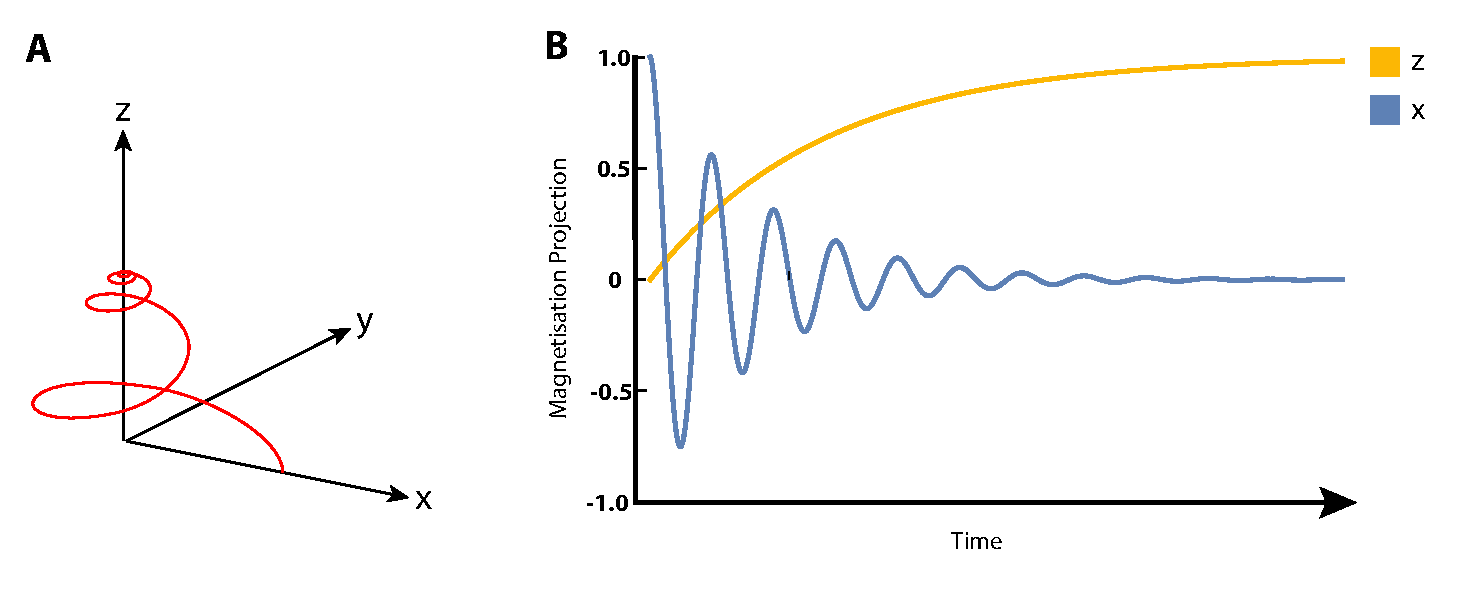
\includegraphics[width=\textwidth]{T1T2.pdf}}
  \caption{A) a magnetisation vector precesses in the $xy$-plane, eventually returning to equilibrium.
  B) A plot of the magnetisation along $z$-axis (yellow) and the $x$-axis (blue) during the relaxation.}
  \label{fig:t1t2}
\end{figure}

Relaxation occurs when the spins exchange energy with their surroundings. They do
this when local magnetic fields, usually caused by the motion of surrounding molecules, oscillate
near the larmour frequency of the relaxing spin. These oscillating fields can be thought of
as local RF pulses we discussed earlier, the key difference is that they only affect a few spins
and not the sample as a whole. Essentially relaxation is an energy exchange between the
spins and the molecules surrounding them. This is the origin of the original name for longitudal
relaxation - spin-lattice relaxation.

\newpage

\subsection{Quantum description of NMR}\label{Quantum}

In this chapter, I will introduce the the quantum description of NMR. Including how
we use operators and superoperators to understand how states change under different conditons and how the energies of the system can be extracted.

\subsubsection{Nuclear Spin}

Nuclear spin can be treated as a type of angular momentum. Spin angular momentum can be characterized by its total
angular momentum, and the angular momentum with respect to a reference axis (usually z).  Denoted by $\hat{I}$
it is comprised of a magnitude, $\lvert\hat{I}\rvert$, and a direction, $m_I$.
The magnitude is given by
\begin{equation}
  \lvert\hat{I}\rvert = \hbar\sqrt{I(I+1)}
\end{equation}
where $\hbar$ is the reduced Planck constant and $I = 0,\frac{1}{2},1,\dots$. The projection of $\hat{I}$ in
the $z$ direction, $\hat{I}_{z}$, is given by
\begin{equation}
  \hat{I}_{z} = m_I\hbar
\end{equation}
$m_{I}$ can take integer values from $-I$ to $+I$ shown in \fig{fig:Projection}

For the commonly occuring case of a spin-1/2 nucleus, $I=1/2$ and $m_I = ±1/2$ and if we were to measure $\hat{I}_z$ we would get a value of  with an associated probability depending which state the system is in. Indicating the possible measurement outcomes for $\hat{I}_z$ are $±\frac{\hbar}{2}$.

\begin{figure}
  \begin{center}
  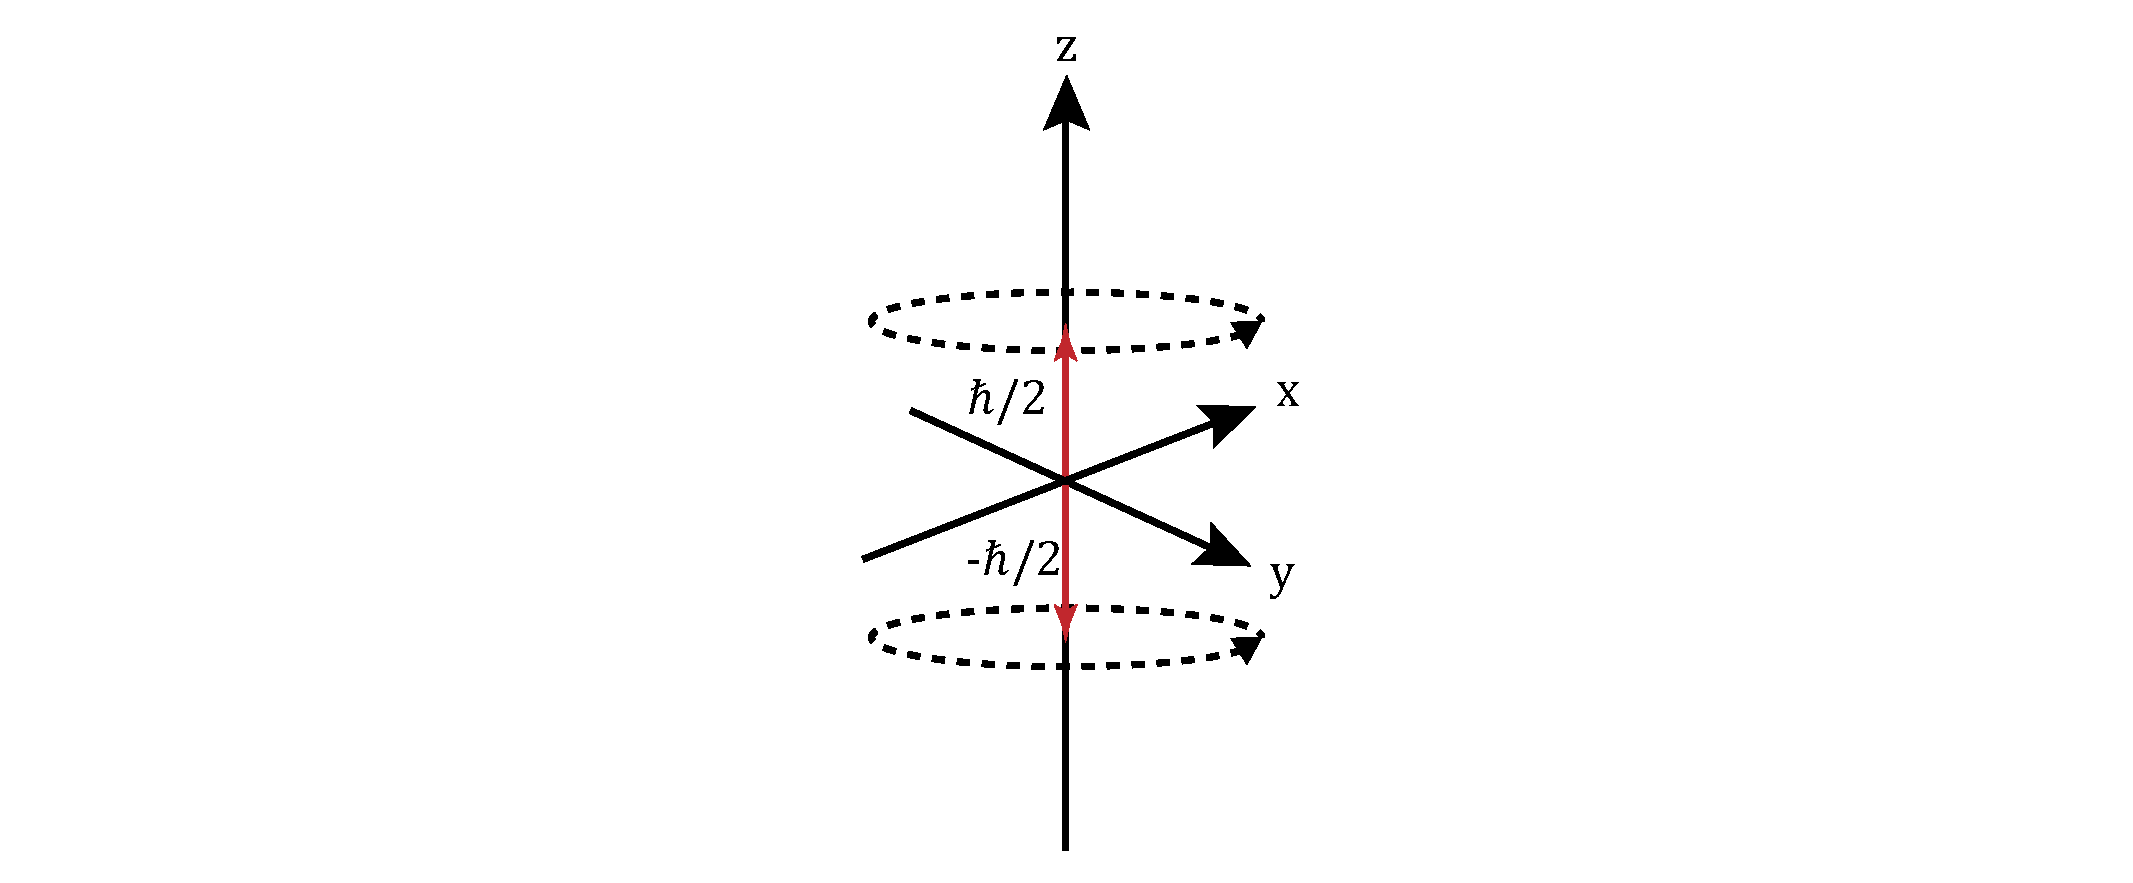
\includegraphics[width=\columnwidth,height=5cm,keepaspectratio]{StateProjection.pdf}
  \end{center}
  \caption{The projection of two states in a spin 1/2 nucleus (red arrow) with the magnitudes indicated (black arrow)}
  \label{fig:Projection}
\end{figure}

\subsubsection{Spin States}\label{SpinStates}

If a spin-1/2 nucleus is placed in a magnetic field (taken to be oriented along $z$) it can be represented using two basis states.
State one has $I = 1/2$, $m_I = 1/2$ and State two has $I = 1/2$, $m_I = -1/2$. We denote these as $\ket{I,m_I}$\citep{dirac_1939}, for simplicity we omit the $I$ and are left with
$\ket{m_I}$. For the special case of a spin-1/2 the two states are known as zeeman states denoted by $\ket{\alpha}$ and $\ket{\beta}$. Where the $\ket{\alpha}$ state has angular momentum +1/2 and $\ket{\beta}$ has -1/2.

The zeeman states take the following form:

\begin{equation}
  \ket{\alpha} = \begin{pmatrix}
    1\\
    0
\end{pmatrix}
 \ket{\beta} = \begin{pmatrix}
   0\\
   1
\end{pmatrix}
\end{equation}

bras are also defined by taking the conjugate transpose of the ket, $\ket{\alpha}^{\dagger} =
\bra{\alpha}$ such that
\begin{equation}
  \bra{\alpha} = \begin{pmatrix}
    1 & 0
\end{pmatrix}
  \bra{\beta} = \begin{pmatrix}
  1 & 0
\end{pmatrix}
\end{equation}

The state, $\ket{\psi}$, of a two level system can now be completely decribed in this basis
as the linear combination of the basis states:
\begin{equation}\label{eqn:zeeman}
  \ket{\psi} = c_1\ket{\alpha} + c_2\ket{\beta} = \begin{pmatrix}
    c_1\\
    c_2
\end{pmatrix}
\end{equation}
\begin{equation}
  \bra{\psi} = c_1^*\bra{\alpha} + c_2^*\ket{\beta} = \begin{pmatrix}
    c_1^* & c_2^*
\end{pmatrix}
\end{equation}

These are normalised such that $c_1c_1^* + c_2c_2^* = 1$.

To complete the picture the sates must me orthonormal. Orthonormality between states exists if
if the inner product of the basis states $\ket{r_i} ~\text{and}~ \ket{r_j}$ satisifies the following conditions:

\begin{equation}
  \langle r_i\vert r_j\rangle = \delta_{ij}
\end{equation}

where the Kronecker delta is:
\begin{equation}
  \delta_{ij} = \begin{cases}
    0 & ~\text{if}~ i \ne j\\
    1 & ~\text{if}~ i = j
                \end{cases}
\end{equation}

where $\langle r_i\vert r_j\rangle = \delta_{ij}$ denotes taking the dot product between the two
vectors $\ket{r_i}$ and $\ket{r_j}$.

The basis states help to quantify the component of a state vector along that state. Take our example from \eqn{eqn:zeeman}, we can construct inner products of the overall state, $\ket{\psi}$ with $\ket{\alpha}$ and $\ket{\beta}$ to determine component of the basis states.
\begin{equation}
  \langle\alpha\vert\psi\rangle = c_1 \quad \langle\beta\vert\psi\rangle = c_2
\end{equation}

The outer product of the basis state, $\ket{r_n}$, for an N-spin system must satisfy:
\begin{equation}
  \sum_{n=1}^{N} \ket{r_n}\bra{r_n} = \mathbb{1}
\end{equation}

where $\mathbb{1}$ is an N by N identity matrix.

When a second spin is introduced, the Hilbert space is extended to accommodate additional spin
states by taking the tensor product of the basis states


\begin{align}\label{eqn:2spinstates}
\ket{\alpha_{1}\alpha_{2}} = \ket{\alpha_1} \otimes \ket{\alpha_2} = \begin{pmatrix}
  1\\
  0\\
  0\\
  0
\end{pmatrix} &\quad
\ket{\alpha_{1}\beta_{2}} = \ket{\alpha_1} \otimes \ket{\beta_2} = \begin{pmatrix}
  0\\
  1\\
  0\\
  0
\end{pmatrix}\\
\ket{\beta_{1}\alpha_{2}} = \ket{\beta_1} \otimes \ket{\alpha_2} = \begin{pmatrix}
  0\\
  0\\
  1\\
  0
\end{pmatrix} &\quad
\ket{\beta_{1}\beta_{2}} = \ket{\beta_1} \otimes \ket{\beta_2} = \begin{pmatrix}
  0\\
  0\\
  0\\
  1
\end{pmatrix}
\end{align}
The subscripts indicate which spin we are reffering to, e.g. $\ket{\beta_1\alpha_2}$ means that
spin 1 is in the $\beta$ state and spin 2 is in the $\alpha$ state.

\subsubsection{Operators}

Operators act on states. To explain this, let's consider a generic operator $\hat{B}$ with eigenstates $\ket{\alpha}$ and $\ket{\beta}$. When a state is acted upon by an operator it is denoted by:
\begin{equation}
  \hat{B}\ket{\alpha} = b\ket{\alpha}
\end{equation}

the same state is returned, multiplied by some scalar $b$, that is an eigenvalue of $\ket{\alpha}$
in the operator basis B.

The expectation value of an operator can be found by:
\begin{equation}\label{eqn:expectation}
  \langle\hat{B}\rangle = \langle\alpha\vert\hat{B}\vert\alpha\rangle = b\langle\alpha\vert\alpha\rangle = b
\end{equation}

this returns the eigenvalue.

In NMR we use three operators to determine the projection of angular momentum along a specific axis, $\hat{I}_x$, $\hat{I}_y$, and $\hat{I}_z$. These are defined by the Pauli matrices multiplied by $\frac{\hbar}{2}$.

\begin{equation}
  \hat{I}_x=\frac{\hbar}{2}\begin{pmatrix}
    0 & 1\\
    1 & 0
\end{pmatrix}\quad
\hat{I}_y=\frac{\hbar}{2i}\begin{pmatrix}
  0 & 1\\
  -1 & 0
\end{pmatrix}\quad
\hat{I}_z=\frac{\hbar}{2}\begin{pmatrix}
  1 & 0\\
  0 & 1
\end{pmatrix}
\end{equation}

as an example, let's take the example from before of a spin-1/2 particle in a magnetic field
and see what happens if we were to project the $\ket{\alpha}$ state along the z-axis.
\begin{equation}\label{eqn:operators}
  \hat{I}_z\ket{\alpha} = \frac{\hbar}{2}\begin{pmatrix}
    0 & 1\\
    1 & 0
\end{pmatrix}
\begin{pmatrix}
  1\\
  0
\end{pmatrix} = \frac{\hbar}{2}\begin{pmatrix}
  1\\
  0
\end{pmatrix} = \frac{\hbar}{2}\ket{\alpha}
\end{equation}
We find that $\frac{\hbar}{2}$ is the eigenvalue of $\ket{\alpha}$ for the operator $\hat{I}_z$. For ease of handling in the following examples we will take $\hbar$ = 1.

We will now examine three more operators and explore how they act on states. They are the total square angular momentum, $\hat{I}^2$ and the two shift operators $\hat{I}^+$ and $\hat{I}^-$ defined as the following:

\begin{align}
  \hat{I}^2 =& \hat{I}_x^2 + \hat{I}_y^2 + \hat{I}_z^2\\
  \hat{I}^+ =& \hat{I}_x + i\hat{I}_y\\
  \hat{I}^- =& \hat{I}_x - i\hat{I}_y
\end{align}
They act on states according to:
\begin{align}
  \hat{I}^2\ket{I,m_I} =& I(I+1)\ket{I, m_I}\\
  \hat{I}^+\ket{I,m_I} =& \sqrt{(I(I+1)-m_I(m_I+1))}\ket{I,m_{I+1}}\\
  \hat{I}^-\ket{I,m_I} =& \sqrt{(I(I+1)-m_I(m_I-1))}\ket{I,m_{I-1}}
\end{align}
Using a spin-1/2 particle in a magnetic field as an example we'll let these operators act on the $\ket{\alpha}$ state
\begin{align}
  \hat{I}^2\ket{\alpha} =& \frac{3}{4}\ket{\alpha}\\
  \hat{I}^+\ket{\alpha} =& 0\\
  \hat{I}^-\ket{\alpha} =& \ket{\beta}\\
  \hat{I}^+\ket{\beta} =& \ket{\alpha}\\
  \hat{I}^-\ket{\beta} =& 0
\end{align}
As the '+' and '-' denote raising or lowering $m_I$ by 1


We can see if two operators commute by using the commutator which is defined as:
\begin{equation}
  [\hat{A},\hat{B}] = \hat{A}\hat{B} - \hat{B}\hat{A}
\end{equation}

If $[\hat{A},\hat{B}] = 0$ the operators are said to commute. The $\hat{I}_z$, $\hat{I}_z$ and $\hat{I}_z$
have cyclic commutation rules:
\begin{align}\label{eqn:commutator}
  [\hat{I}_x,\hat{I}_y] = i\hat{I}_z\\
  [\hat{I}_y,\hat{I}_z] = i\hat{I}_x\\
  [\hat{I}_x,\hat{I}_z] = i\hat{I}_y
\end{align}

These relationships are important in NMR as they help govern the rules for the rotations of spins.

\subsubsection{Superoperators}

Like states, that can be transformed by operators, we can define objects that act in a similar manner on operators. These objects are called superoperators.

To start, let's take a simple commutation superoperator, $\hat{\hat{A}}$, defined as:
\begin{equation}
  \hat{\hat{A}}\hat{B} = [\hat{A},\hat{B}] = \hat{A}\hat{B} - \hat{B}\hat{A}
\end{equation}
Applying it to operator $\hat{B}$ results in the commutation of $\hat{A}$ and $\hat{B}$

In NMR, three rotational superoperators can be defined using the commutation superoperators from \eqn{eqn:operators}:
\begin{equation}
 \hat{\hat{R}}_x(\theta) = \text{exp}\{-i\hat{\hat{I}}_x\theta\}\quad\hat{\hat{R}}_y(\theta) = \text{exp}\{-i\hat{\hat{I}}_y\theta\}\quad\hat{\hat{R}}_z(\theta) = \text{exp}\{-i\hat{\hat{I}}_z\theta\}
\end{equation}

These are applied to to the angular momentum operators using the sandwich formula:
\begin{equation}
  \hat{\hat{R}}_x(\theta)\hat{I}_z = \text{exp}\{-i\hat{\hat{I}}_x\theta\}\hat{I}_z\text{exp}\{+i\hat{\hat{I}}_x\theta\}
\end{equation}

The result of this is a rotation of $\hat{I}_z$ around the $x$-axis by an angle $\theta$:
\begin{equation}
  \hat{\hat{R}}_x(\theta)\hat{I}_z = \cos{\theta}\hat{I}_z - \sin{\theta}\hat{I}_y
\end{equation}

The rotational direction (sign of the $\sin{\theta}$ term) is determined by the right hand co-ordinate system defined in \eqn{eqn:commutator}.

We will now discuss how these are used in describing the spin dynamics of a spin system.

\subsubsection{Density Operator}

The density operator is a description of an ensemble of spin sytems.

Let's go back once again to a spin-1/2 particle in a magnetic field. Where $\ket{\psi}$ is some superposition state in the two level system such that:
\begin{align}
\ket{\psi} =& \begin{pmatrix}
    c_1\\
    c_2
\end{pmatrix} = c_1\ket{\alpha} + c_2\ket{\beta}\\
\bra{\psi} =& \begin{pmatrix}
  c_1^* & c_2^*
\end{pmatrix} = c_1^*\bra{\alpha} + c_2^*\bra{\beta}
\end{align}

The density operator has the form:
\begin{equation}
  \hat\rho = \overline{\ket{\psi}\bra{\psi}} = \begin{pmatrix}
    \overline{c_1c_1^*} & \overline{c_1c_2^*}\\
    \overline{c_2c_1^*} & \overline{c_2c_2^*}
\end{pmatrix}
\end{equation}
Where $\overline{\ket{\psi}\bra{\psi}}$ denotes the ensemble average.

If the number of spins is increased, the denstiy operator's form does not change instead it provides
an average for the entire ensemble of spin states. The population of a given state is given by the expectation
value of the density operator as in \eqn{eqn:expectation}. If we would like to know
the population of state $\ket{\alpha}$ we would perform the following:

\begin{equation}
  \langle\alpha\vert\hat\rho\vert\alpha\rangle = \overline{\langle\alpha\vert\psi\rangle} \overline{\langle\alpha\vert\psi\rangle} = \overline{c_1^*c_1}
\end{equation}

The diagonal elements of $\hat\rho$ are state populations or the probabilities of being in a certain state.

The off-diagonal elements are coherences between states. These coherences represent superposition These coherences are complex numbers and two coherences between the same pair of states are complex cojugates of each other. e.g.:
\begin{equation}
  \langle\alpha\vert\hat\rho\vert\beta\rangle = (\langle\beta\vert\hat\rho\vert\alpha\rangle)^* = c_1c_2^* = (c_1^*c_2)^*
\end{equation}
The coherence order between two states in a magnetic field is defined as the difference in angular
momentum projection along the $z$ axis. In our two spin this would be(with $\hbar = 1$):
\begin{align}
  \hat{I}_z\ket{\beta} = m_\alpha = +\frac{1}{2}\ket{\alpha}\\
  \hat{I}_z\ket{\beta} = m_\beta = -\frac{1}{2}\ket{\beta}
\end{align}
We can use these results to calculate the coherence order of the coherence $\langle\alpha\vert\hat\rho\vert\beta\rangle$:
\begin{equation}
 m_\alpha - m_\beta = +1
\end{equation}
and conversely the coherence order of $\langle\beta\vert\hat\rho\vert\alpha\rangle$ is:
\begin{equation}
  m_\beta - m_\alpha = -1
\end{equation}

Now let's look at how $\hat\rho$ relates to the angular momentum operators given in \eqn{eqn:operators}.

Usually in NMR there are $>10^{20}$ spins in the sample, the density operator becomes more advantageous here
as mentioned it contains information about the entire spin ensemble. Normally, there is only a small population difference between $\alpha$ and $\beta$ (see \ref{Population}),
but for this example let's imagine we have found a sufficiently strong enough field for a population difference of $0.1$. The density operator in this case would be:
\begin{equation}
  \hat\rho = \frac{1}{2}\begin{pmatrix}
    1 + 0.1 & 0\\
    0 & 1-0.1
\end{pmatrix}
\end{equation}
using the definition given in \eqn{eqn:operators} we can re-write this as
\begin{equation}
  \hat\rho = \frac{1}{2}\hat{\mathbb{1}} + 0.1\hat{I}_z
\end{equation}
$\hat{\mathbb{1}}$ is identity matrix and corresponds to no population difference between $\ket{\alpha}$ and $\ket{\beta}$.

$\hat{\mathbb{1}}$ is unaffected by rotations so can be ignored in the context of NMR
and so we write
\begin{equation}
  \hat{\rho} = 0.1\hat{I}_z
\end{equation}
to describe the $z$ magnetisation of our sample.

The density operator can also be used to to describe the evolution of a spin system under operations. If we applied a $90$ degree pulse along the $y$ axis, denoted using radians by $(\pi/2)_y$. That is the equivalent of propagating the initial density operator, $\rho_0$
under the rotation superoperator $\hat{\hat{R}}_y(\pi/2)$:
\begin{equation}
  \hat{\rho}_1 = \hat{\hat{R}}_y(\frac{\pi}{2})\hat\rho_0 = \text{exp}\{-i(\frac{\pi}{2})\hat{\hat{I}}_y\}\hat{I}_z\text{exp}\{+i(\frac{\pi}{2})\hat{\hat{I}}_y\} = \hat{I}_x
\end{equation}
Now the magnetisation is in the $x$-axis it will begin to precess about the $z$-axis which using our notation is the equivalent of of propagating $\hat{I}_x$ ($\hat{\rho}_1$)
under $\hat{\hat{R}}_z(\omega t)$:
\begin{align}\label{eqn:propagate}
  \hat{\rho}_2 = \hat{\hat{R}}_z(\omega t)\hat{\rho}_1 =& \text{exp}\{-i\omega t\hat{\hat{I}}_z\}\hat{I}_x\text(exp)\{+i\omega t\hat{\hat{I}}_z\}\\
   =& \cos(\omega t)\hat{I}_x + \sin(\omega t)\hat{I}_y
\end{align}
where $\omega$ is the larmour frequency, and $t$ is time.

the $\text{exp}\{i\omega t\}$ is called a propagator, because it propagates the density operator in time.

The Hamiltonian, the energy operator, describes how the system evolves in time and uses progators, rotational superoperators and the density operator in order to do so.

\subsubsection{The Hamiltonian}\label{Hamiltonian}

If we let $\ket{\psi_1}$ and $\ket{\psi_2}$ be eigenstates of the Hamiltonian $\hat{H}$ then
\begin{align}
  \hat{H}\ket{\psi_1} = E_1\ket{\psi_1}\\
  \hat{H}\ket{\psi_2} = E_2\ket{\psi_2}
\end{align}

The Hamiltonian can also be expressed in matrix form:
\begin{equation}
  \hat{H} = \begin{pmatrix}
    E_1 & 0\\
    0 & E_2
\end{pmatrix}
\end{equation}
If the Hamiltonian is written in the eigenbasis of the system its main diagonal correspond to state energies and it has values of $0$ everywhere else.

The evolution in time of a quantum system is described by the Schr\"odinger equation:
\begin{equation}
  i\hbar\frac{\partial}{\partial{t}}\ket{\psi} = \hat{H}\ket{\psi}
\end{equation}
The $\hbar$ was included for completeness sake and will again be set to equal $1$.

In NMR we describe the dynamics of a system using the density operator evolution rather than the evolution of the states using
\begin{align}
  \frac{\partial}{\partial{t}}\ket{\psi} = -i\hat{H}\ket{\psi}\\
  \frac{\partial}{\partial{t}}\bra{\psi} = i\bra{\psi}\hat{H}
\end{align}

we can derive\citep{Neumann2018}:
\begin{align}
  \frac{\partial}{\partial{t}}\hat\rho\quad=&\quad \frac{\partial}{\partial{t}}[\ket{\psi}\bra{\psi}]\\
  =&\quad[\frac{\partial}{\partial{t}}\ket{\psi}]\bra{\psi} + \ket{\psi}[\frac{\partial}{\partial{t}}\bra{\psi}]\\
  =&\quad-i\hat{H}\ket{\psi}\bra{\psi} + i\ket{\psi}\bra{\psi}
\end{align}
to give the relationship
\begin{equation}
  \frac{\partial}{\partial{t}}\hat\rho = -i[\hat{H},\hat\rho]
\end{equation}
this is called the Liouville von Neumann equation.

Returning to our spin-1/2 particle in a magnetic field. The Hamiltonian is initially
proportional to the $z$ angular momentum operator
\begin{equation}
  \hat{H} = \omega\hat{I}_z
\end{equation}

where $\omega = -\gamma B_0$. In matrix form, in our original zeeman basis, the Hamiltonian is:
\begin{equation}
  \hat{H} = \begin{pmatrix}
+\frac{\omega}{2} & 0\\
0 & -\frac{\omega}{2}
\end{pmatrix}
\end{equation}
where
\begin{equation}
  \hat{H}\ket{\alpha} = +\frac{\omega}{2}\ket{\alpha}
\end{equation}

The density operator evolves under a Hamiltonian like so:
\begin{equation}
  \hat\rho(t) = \text{exp}\{-i\hat{H}t\}\hat\rho(0)\text{exp}\{+i\hat{H}t\}
\end{equation}

In \eqn{eqn:propagate}, we saw that the precession of a spin-1/2 particle in a magnetic field can be described using the rotation superoperator around the $z$-axis $\hat{\hat{R}}_z(\omega t)$. We know that for this system its analagous to $\hat{H} = \omega\hat{I}_z$.

If the density operator commutes with the Hamiltonian there is no evolution of the system.
This can be seen more clearly using propagators with $\hat{H} = \omega\hat{I}_z$ and $\rho(0) = \hat{I}_z$
\begin{equation}
  \rho(t) = \text{exp}\{-i\omega t\hat{\hat{I}}_z\}\hat{I}_z\text{exp}\{+i\omega t\hat{\hat{I}}_z\} = \hat{I}_z
\end{equation}
If the density operator does not commute with the Hamiltonian it will evolve. To demostrate this we use $\hat{H} = \omega\hat{I}_z$ as before  however this time $\hat\rho(0) = \hat{I}_x$
\begin{equation}
  \hat\rho(t) = \text{exp}\{-i\omega t\hat{\hat{I}}_z\}\hat{I}_x\text{exp}\{+i\omega t\hat{\hat{I}}_z\} = \cos(\omega t)\hat{I}_x + \sin(\omega t)\hat{I}_y
\end{equation}
The Hamiltonian for multi-spin system is slightly more complicated. Consider a two spin
system $I_1$ and $I_2$ with $J$-coupling $J_{12}$ the Hamiltonian then becomes:
\begin{equation}
  \hat{H} = \omega_1\hat{I}_1 + \omega_2\hat{I}_2 + 2\pi J_{12}\hat{\mathbf{I}}_1\cdot\hat{\mathbf{I}}_2
\end{equation}
where $\hat{\mathbf{I}}_1\cdot\hat{\mathbf{I}}_2 = \hat{I}_{1x}\hat{I}_{2x} + \hat{I}_{1y}\hat{I}_{2y} + \hat{I}_{1z}\hat{I}_{2z}$.
In matrix form in the zeeman basis this is:
\begin{equation}
  \hat{H} = \frac{1}{2}\begin{pmatrix}
    +\omega_1 + \omega_2 + \pi J_{12} & 0 & 0 & 0\\
    0 & +\omega_1 - \omega_2 - \pi J_{12} & 2\pi J_{12} & 0\\
    0 & 2\pi J_{12} & -\omega_1 + \omega_2 - \pi J_{12} & 0\\
    0 & 0 & 0 & -\omega_1 - \omega_2 - \pi J_{12}
\end{pmatrix}
\end{equation}

The zeeman basis is no longer an eigenbasis of the Hamiltonian because the $J$-coupling
introduces off-diagonal terms. In practice, when $|\omega_1-\omega_2| >> 2\pi J_{12}$
these terms are ignored because the zeeman basis is approxiamely the eigen basis of the Hamiltonian. This is termed the secular approxiamation.

However, when this is not the case, the Hamiltonian requires diagonalisation which is beyond the scope of this introduction.

\newpage

\section{Micro-NMR}\label{Micro-NMR}

All NMR experiments depend on two performance metrics: sensitivity and resolution. Sensitivity
here means the minimum number of spins needed to give a signal clearly above the noise. Resolution
quantifies how well different spins in the sample can be differentiated. These two properties
are often linked, by selecting a smaller sample it is possible to enhance resolution by detecting
a smaller portion of spins in the sample but this compromises sensitivity as the number of spins become more
limited.

 In NMR, the long life time of the nuclear spin states (minutes in some cases) contirbute to extremely
 narrow lines in the spectrum with resolutions of one part per billion regularly acheived in
 commercial systems.

 \subsection{Sensitivity}

 \subsubsection{Signal to noise ratio}


 Sensitivity in NMR at thermal equilibrium is always in short supply. In an NMR experiment the signal
 is proportional to the net magnetisation, $M_0$, of the sample\citep{webb2005nmr}:
\begin{equation}\label{eqn:Webb}
  M_0 = \frac{\gamma~h}{4\pi}(I(I+1))(P_{\alpha}-P_{\beta}) = N\gamma^2\hbar^2I(I+1)\frac{B_0}{3k_BT}
\end{equation}
where $\gamma$ is the gyromagnetic ratio of the nucleus,$\hbar$ is Planck's constant $h$/2$\pi$, $P_{\alpha}-P_{\beta}$
is the population difference between zeeman energy levels seen in \ref{Population}, $B_0$ is the magnetic field, $N$ is
the number of spins per unit volume , $k_B$ is the Boltzmann constant and T is the absolute temperature. The magnetisation
and therefore signal depends on the population difference which at room temperature is on the order of $10^{-25}$J
which is much lower that the thermal energy of the system. From the equation, increasing $B_0$ would seem a
valid strategy and comparatively it can be, increasing from 14.1T to 23.5T can almost double the signal,
however even at 23.5T there is only a factor of ~$6\times10^{-6}$ in population difference. It's this
very small value that is responsible for the low sensitivity of NMR compared to other techniques.

Detection in NMR is typically done through the induction of a voltage in a coil that's close
to the precessing nuclear spins this is usually referred to as the sample coil. Unfortunately,
this coil also brings with it a type of interference, noise, analagous to the 'hiss' in the backgound
of radio it is produced mainly from thermal motion of electrons in the sample coil with some contribution from thermal
motion of ions in solution. The signal to noise ratio, SNR, is an important factor in NMR experiments if its too low
the signal will never be seen.

The SNR was formulated by Abragam\citep{Abragam:1961vg} and the analysis extended by Hoult and
Richards\citep{Hoult:1976dw} and is defined as the peak signal divided by the root mean square (rms) noise. By including
the magnetisation from \eqn{eqn:Webb} we find \citep{vanBentum:2007fda}:
\begin{equation}\label{eqn:SNR}
  \text{SNR} = \frac{k_0\frac{B_1}{i}V_s\omega_0\frac{1}{\sqrt{2}}M_0}{F\sqrt{4k_BTR_{\text{noise}}\Delta~f}}
\end{equation}
where $k_0$ is a contant that accounts for spatial inhomogeneities in the $B_1$ field, $V_s$ is the sample volume,
$\omega_0$ is the larmour frequency, the factor $\frac{1}{\sqrt{2}}$ is introduced as the noise is rms noise. The
factor $B_1/i$ the magnetic field from the coil per unit current is defined as the coil sensitivity. The denominator is
the noise determined by the noise factor from the spectrometer ($F$) and the dissipative loses ($R_{\text{noise}}$) of
the coil, circuit and sample for the spectral bandwidth $\Delta~f$. $T$ is the absolute temperature and $k_b$ is the
boltzmann constant.

In the same paper, Hoult and Richards introduced the principle of reciprocity for calculating the
sensitivity of the RF coil, This states that the signal received from a sample by a coil is proportional to the magnetic
field which would have been created in the sample if unit current were passed through the coil. Therefore the SNR is
directly proportional to the sensitivity of the coil, $B_1/i$. This can be seen if we define an
effective sample volume $V'_s = k_0V_s$ that is the volume in which $B_1$ is within 10\% of the maximum
value at the center of the coil. The SNR is given by a more simple expression\citep{vanBentum:2007fda}:
\begin{equation}
  SNR = C\frac{B_1N_s}{i\sqrt{R\Delta~f}}
\end{equation}
where $N_s$ is the number of spins in located within an effective volume $V'_s$.
For protons at 600MHz the constant, $C$ equals $1.4\times10^{-11}$ in SI units ($B_0$ = 14.1T, $T$ = 300K, $\gamma$ =
$0.2675\times10^9$ $\text{rad} \text{T}^{-1}\text{s}^{-1}$, $I = 1/2$ and $F = 1$ assuming neglible noise from the spectrometer.)

From the simple expression it becomes clear that the way to improve SNR is to increase the filling factor
(optimize the number of spins in the number of spins in $B_1$), maximise coil sensitivity, $B_1/i$, and
minimise the total resistance. The filling factor, $\alpha_F$ is given by:
\begin{equation}\label{eqn:FillingFactor}
  \alpha_F = \frac{\int~B_1^2\rho(r)dV}{\int~B_1^2dV}
\end{equation}
where the function $\rho$ is unity in the sample area, and zero elsewhere. For a long solenoid coil with the
interior space filled with sample, $\alpha_F = 1/2$. Most other desings have a lower filling factor.

Two of these three can be solved by decreasing the size of the detector. The third, minimising resistance
can be tackled by commercially available cryoprobes where the coil is cooled with a stream of He gas to
~20K this reduces the thermal noise from the source and can increase SNR by a factor of four.

To see how size of coil affects SNR we take an RF helical coil. An idealised coil
is a cylindrical shell with uniform current density. The RF current penetrates to a frequency
specific depth $\delta$. For copper at 600 MHz and room temperature $\delta$ = 2.7 $\mu$m. The center
field is given by:
\begin{equation}
  \frac{B_1}{i} = \frac{\mu_0}{\sqrt{l^2+d^2}}
\end{equation}
Resistance is:
\begin{equation}
  R = \rho\frac{\pi~d}{l\delta}
\end{equation}
with l, the height of the copper cylinder, d the diameter and $\rho$ the resistivity.
Optimum coil sensitivity is given by $d/l$ = $1$ in this case the signal to noise is:
\begin{equation}
  SNR = 0.9\times10^{-16}\frac{N_s}{d\sqrt{\Delta~f}}
\end{equation}
For a fixed number of spins the SNR scales with 1/d as predicted by \citep{Hoult:1976dw}

\subsection{Limit of Detection}

The signal to noise ratio can be found in the time or frequency domain. In the time domain the noise, $N$, is proportional to
$\sqrt{\Delta~f}$. Therefore the SNR in the time domain is not a good measure of sensitivity, it can be
artificially inflated by narrowing the bandwidth. Instead it is better to use \textit{limit of deteciton}, deined as
the number of spins that have to resonate within a bandwidth of 1 Hz to give an SNR of 3. This gives
the normalised limit of detection as\citep{Badilita:2011td}:
\begin{equation}
  \text{nLOD}_{t} = \frac{3n_s}{\text{SNR}_{t}\sqrt{\Delta~f}}
\end{equation}
Where $n_s$ is the number of spins that were present in the sample for the measurement and $\text{SNR}_t$ is the
signal to noise ratio in the time domain.
In the frequency domain, this becomes
\begin{equation}\label{eqn:nLOD}
  \text{nLOD}_\omega = \frac{3n_s\sqrt{\Delta~t}}{\text{SNR}_\omega}
\end{equation}
here, $\Delta~t$ is the effective acquisition time for a single scan given by the inverse of the
line broadening applied in the processing of the spectrum.

Practically, NMR relies on signal averaging (see \ref{Signal Averaging}) to enhance the spectra. This
method requires waiting between scans for the spins to reach thermal equilibrium. In
this case, a better measure of sensitivity can be applied by using total measurement time
as $\Delta~t$. The drawback here, is that the limit of detection now depends on instrumentation
and sample as $T_1$ relaxation dictates the experiment repetition rate.

\subsection{Concentration limit of detection}

Both types of LOD discussed so far are absolute measures. It is often of more
interest to examine the \textit{concentration} limit of detection cLOD. This is given by
dividing the LOD by the sample volume:
\begin{equation}\label{eqn:cLOD}
  \text{cLOD} = \frac{nLOD}{V_s} = \frac{\text{nLOD}}{\alpha_fV_c}
\end{equation}
Where $V_c$ is the volume of the coil and $\alpha_f$ is the filling factor defined in \eqn{eqn:FillingFactor}.

\eqn{eqn:SNR} and \eqn{eqn:Webb} show that overall the SNR and
magnetisation depend on number of spins and energy level population differences, therefore, best practice
would be to wherever possible have higher $B_0$ to increase population differences and in the case of
concentrated limited samples to have a larger volume, increasing the number of spins.
One of the major reasons, however, for development of micro-NMR has been the scaling of SNR and thefore LOD
with coil size. The trade off here is that as the coil size, and LOD, becomes lower and lower, the
volume shrinks too which leads to losses in cLOD. Micro-NMR therefore, only makes sense for mass
or volume limited samples.


\subsection{Transmission line probe}

This work employs the use of a planar transmission line probe(TLP)\citep{Finch:2016gv, RN164}, in which the geometry
differs from that of a classic micro-coil. The design of which is based off early work by van Bentum \textit{et
al.} and for an equivalent helix gives $\sqrt{2}$ larger SNR\citep{vanBentum:2007fda}. The design of the TLP is shown in
\fig{fig:MVProbe}. It works with a generic microfluidic device that has well defined outer geometry and a fixed sample
chamber position.
\begin{figure}
  \begin{center}
  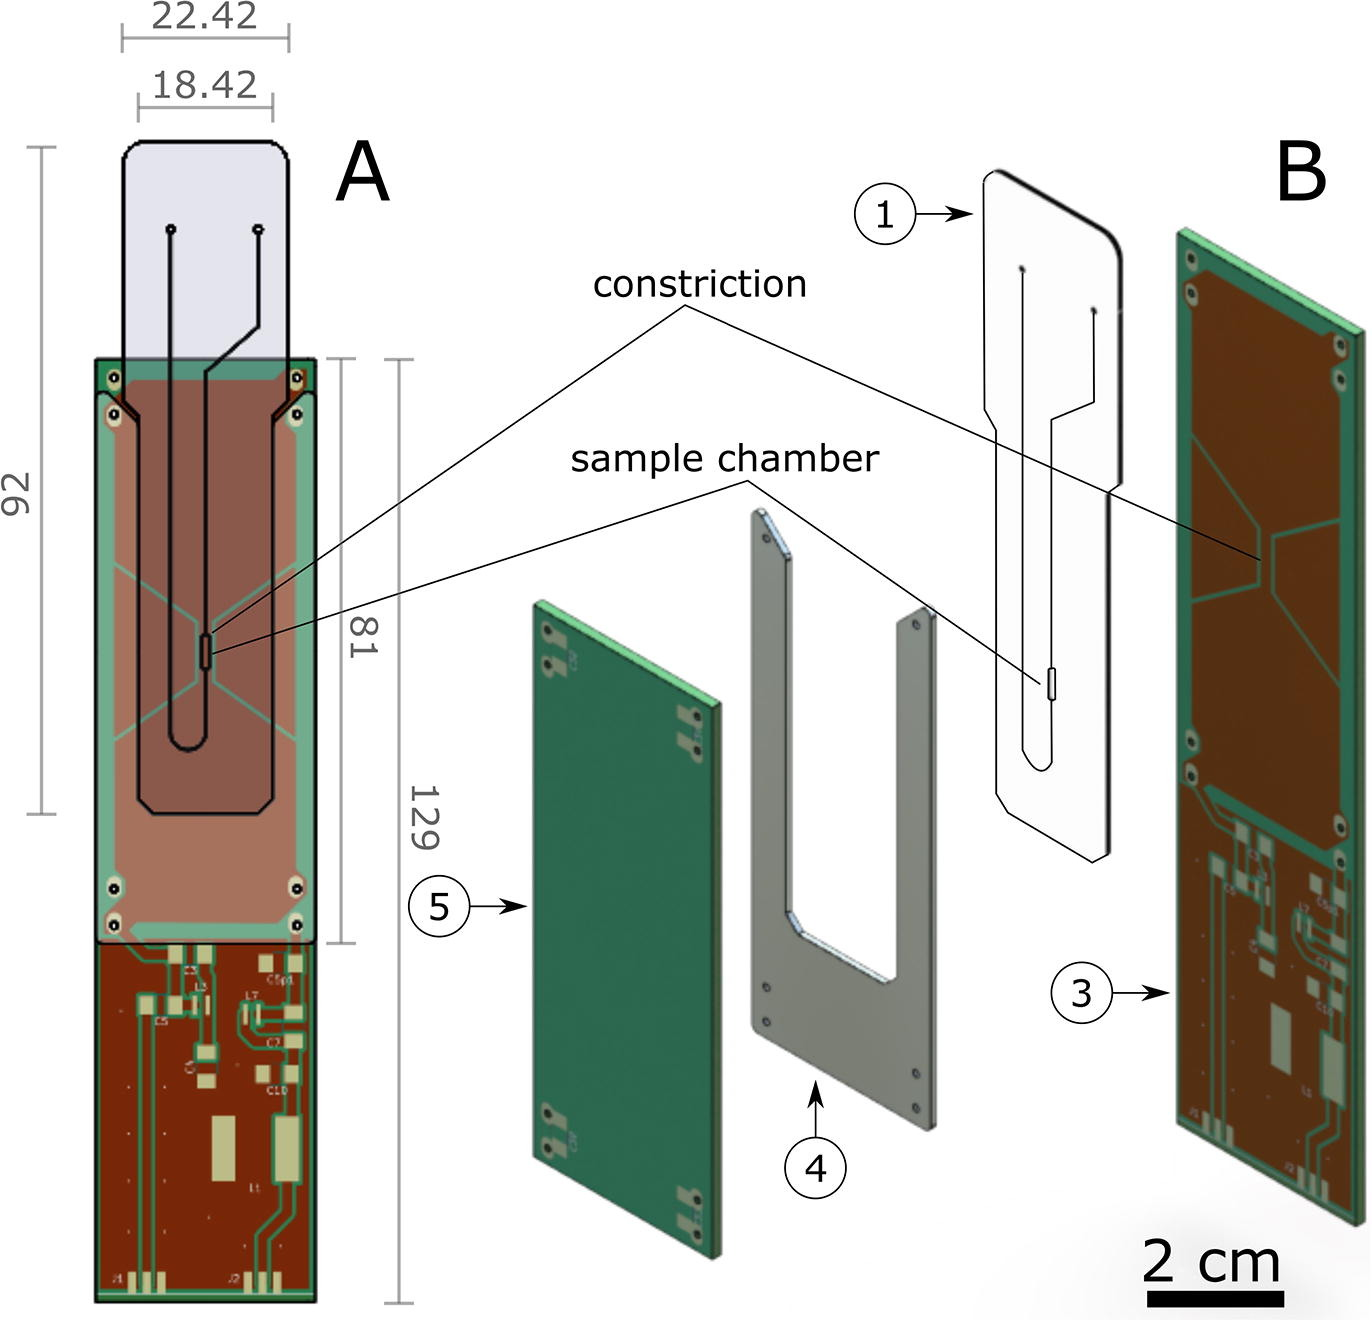
\includegraphics[width=\columnwidth]{Manvendra-Probe.jpg}
  \end{center}
  \caption{Drawings of the detector assembly and the microfluidic device (1). A: front view (dimensions in mm); B:
  exploded view. Spacer (4) ensures the alignment of the sample chamber with the constrictions on the PCB planes. In A,
  PCB plane 5 is hidden to show the orientation of 1 with respect to PCB plane 3. Thickness of each of the PCB planes
  is 1.52 mm and the copper layers on the PCBs is 35 $\mu~\text{m}$. Both the microfluidic device and the spacer are made from
  PMMA and have thickness of 0.9 mm and 1 mm respectively. Figure reproduced from\citep{RN164}}
  \label{fig:MVProbe}
\end{figure}
The main advantage of using this probe is the compatibility of the device with customisable chips allowing
a broad range of applications and enabling the marrying of practical NMR and some microfluidic capabilities which
few others allow\citep{RN165,RN166,RN167}. The limit of detection LOD for the TLP used is
1.4 nmol $\text{s}^{1/2}$ which comparitavely lower than detectors of a similar size and more similar to the LOD of
commercial cryo-probes mentioned previously. Where the probe is exceptional in terms of micro-detector is
the cLOD. Demonstrated in \fig{fig:cLOD}.
\begin{figure}
  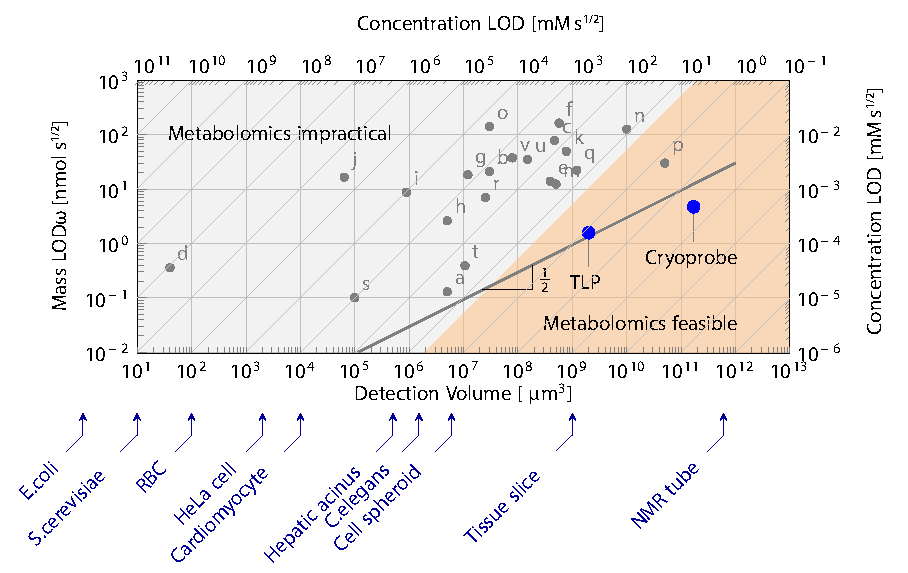
\includegraphics[width=\columnwidth]{sensitivity-ov.pdf}
  \caption{Plot comparing the limits of detection of previously design micro-NMR detectors. Letters
  a-t correspond to different authors as cited by Badilita \textit{et al.}\citep{Badilita:2011td} Letters u\citep{Meier:2014ds}
  and t\citep{RN165} represent more recent work. The probe used here is labelled at TLP and a comercial cyroprobe is shown for reference.}
  \label{fig:cLOD}
\end{figure}

For this work, the goal is not only to combine NMR detection and microfluidics, clearly that has been done before. However,
it is the combination of these two in a way that does not comprimise in either. That, in an NMR sense, means nLODs
comparible to macroprobes as well as sub 0.01 ppm line widths for true spectral resoltuion. This is displayed in
\fig{fig:cLOD}, the area shaded orange that we define as the 'metabolomics feasible' range is a maximum 5 mM $\sqrt{\text{s}}$
ensuring species present at 0.1 mM can be detected within less than 20 mins to a sufficient resolution. The TLP has a cLOD of
~ 1 mM $\sqrt{\text{s}}$ and can detect species at 0.02 mM in that time frame Whilst this is suitable for some metabolomic information to be
gained, however, the subtle changes in molecules present at less than 0.02 mM still evades us in the given time frame. Efforts towards
lowering the nLOD and cLOD are described in \ref{Chapter:Parahydrogen}
